\documentclass[a4paper]{report}
\usepackage[utf8]{inputenc}
\usepackage{amsmath}
\usepackage{esint}
\usepackage{tabstackengine}
\usepackage[colorlinks,linkcolor=blue]{hyperref}
\usepackage{xeCJK}
\usepackage{mathrsfs}
\usepackage{commath}
\usepackage{tikz}
\usepackage{float}
\usetikzlibrary{calc}
\usepackage{pgfplots}
\usepackage{mathrsfs}
\usetikzlibrary{arrows}
\usepackage{pgf,tikz,pgfplots}
\usepackage{ulem}
\usepackage{graphicx}
\usepackage{amsfonts}
\graphicspath{ {../resources/figure/rf/} }
%%%% 下面的命令重定义页面边距,使其符合中文刊物习惯 %%%%
\addtolength{\topmargin}{-54pt}
\setlength{\oddsidemargin}{0.63cm}  % 3.17cm - 1 inch
\setlength{\evensidemargin}{\oddsidemargin}
\setlength{\textwidth}{14.66cm}
\setlength{\textheight}{24.00cm}    % 24.62

%%%% 段落首行缩进两个字 %%%%
% \makeatletter
% \let\@afterindentfalse\@afterindenttrue
% \@afterindenttrue
% \makeatother
% \setlength{\parindent}{2em}  %中文缩进两个汉字位

% 段首不缩进
\setlength{\parindent}{0pt}
%%%% 下面的命令设置行间距与段落间距 %%%%
\linespread{1.4}
% \setlength{\parskip}{1ex}
\setlength{\parskip}{0.5\baselineskip}

\title{Note}
\author{Crosstyan}
\date{July 2020}

\begin{document}
\chapter{Introduction}
\section{波与频率}
% Table generated by Excel2LaTeX from sheet 'Sheet1'
\begin{table}[htbp]
  \centering
  \caption{波长与频率关系}
  \resizebox{\textwidth}{!}{
    
    \begin{tabular}{cclcll}
    频段名称  & 缩写    & \multicolumn{1}{c}{频率范围} & 波段    & \multicolumn{1}{c}{波长范围} &  \\
    \hline
    极低频   & ELF   & 3-30 赫兹(3Hz–30Hz) & 极长波   & 100,000千米 – 10,000千米 &  \\
    超低频   & SLF   & 30–300 赫兹(30Hz–300Hz) & 超长波   & 10,000千米 – 1,000千米 &  \\
    特低频   & ULF   & 300–3000 赫兹(300Hz–3KHz) & 特长波   & 1,000千米 – 100千米 &  \\
    甚低频   & VLF   & 3–30 千赫(3KHz–30KHz) & 甚长波   & 100千米 – 10千米 &  \\
    低频    & LF    & 30–300 千赫(30KHz–300KHz) & 长波    & 10千米 – 1千米 &  \\
    中频    & MF    & 300–3000 千赫(300KHz–3MHz) & 中波    & 1千米 – 100米 &  \\
    高频    & HF    & 3–30 兆赫(3MHz–30MHz) & 短波    & 100米 – 10米 &  \\
    甚高频   & VHF   & 30–300 兆赫(30MHz–300MHz) & 米波    & 10米 – 1米 &  \\
    特高频   & UHF   & 300–3000 兆赫(300MHz–3GHz) & 分米波   & 1米 – 100毫米 &  \\
    超高频   & SHF   & 3–30 吉赫(3GHz–30GHz) & 厘米波   & 100毫米 – 10毫米 &  \\
    极高频   & EHF   & 30–300 吉赫(30GHz–300GHz) & 毫米波   & 10毫米 – 1毫米 &  \\
    太赫兹辐射 & THF   & 0.3-3 太赫兹(0.3THz–3THz) & 亚毫米波  & 1毫米 – 0.1毫米 &  \\
    \end{tabular}%
  }
\end{table}%
$$v_p=f\lambda$$
\begin{figure}[h]
\centering
\resizebox{\textwidth}{!}{

\begin{tikzpicture}
  \tikzset{
    box/.style={draw, rectangle, fill=blue!20, rounded corners, minimum height=3em, node distance=3cm},
    osc/.style={draw, circle, fill=green!20, minimum height=3em, node distance=3cm},
    amp/.style={draw, rectangle, fill=red!20, node distance=4cm},
    line/.style={draw, -latex'}
  }
  \node [box] (mod) {Modulation};
  \node [osc, below of =mod] (osc1) {OSC};
  \node [amp, right of = mod] (amp1) {Hi-freq Power AMP};
  \node [amp, right of = amp1, node distance=5cm] (amp2) {Hi-freq Small AMP};
  \node [box, right of = amp2, node distance = 4cm] (demod) {Demodulation}; 
  \node [osc, below of = demod] (osc2) {OSC};
  
  \path [line] (osc1)--(mod);
  \path [line] (mod)--(amp1);
  \path [line,dashed] (amp1)--node[above]{EM Wave} (amp2);
  %yshift
  \path [line] (amp2)--(demod);
  \path [line] (osc2)--(demod);
  \end{tikzpicture}
}
\caption{信号的传输}
\end{figure}
\chapter{选频网络}
\section{电容和电感}
\begin{align*}
  i&=C\cdot \frac{d v }{d t} &&\text{电容}\\
  v&=L\cdot \frac{d i }{d t} &&\text{电感}
\end{align*}
电容的电压滞后90\textdegree, 电感的电压超前90\textdegree. 
\footnotetext{$\frac{1}{j}=-j$}
\begin{align*}
  \mathbb{Z}_C&=\frac{1}{j\omega C}=-j\cdot\frac{1}{\omega C}&&\text{电容\footnotemark}\\
  \mathbb{Z}_L&=j\omega L &&\text{电感}
\end{align*}
电感品质因数(Q值)
$$Q=\frac{\omega L}{R}$$
Q值越高, 储能越强, 功率损耗越小, 电路效率越高. 
\subsection{电感等效模型}
电感器可以等效为电感$L$串联损耗电阻$R$ (这个损耗电阻一般是不可被忽略的)
\section{Serial}
\begin{figure}[h]
\centering
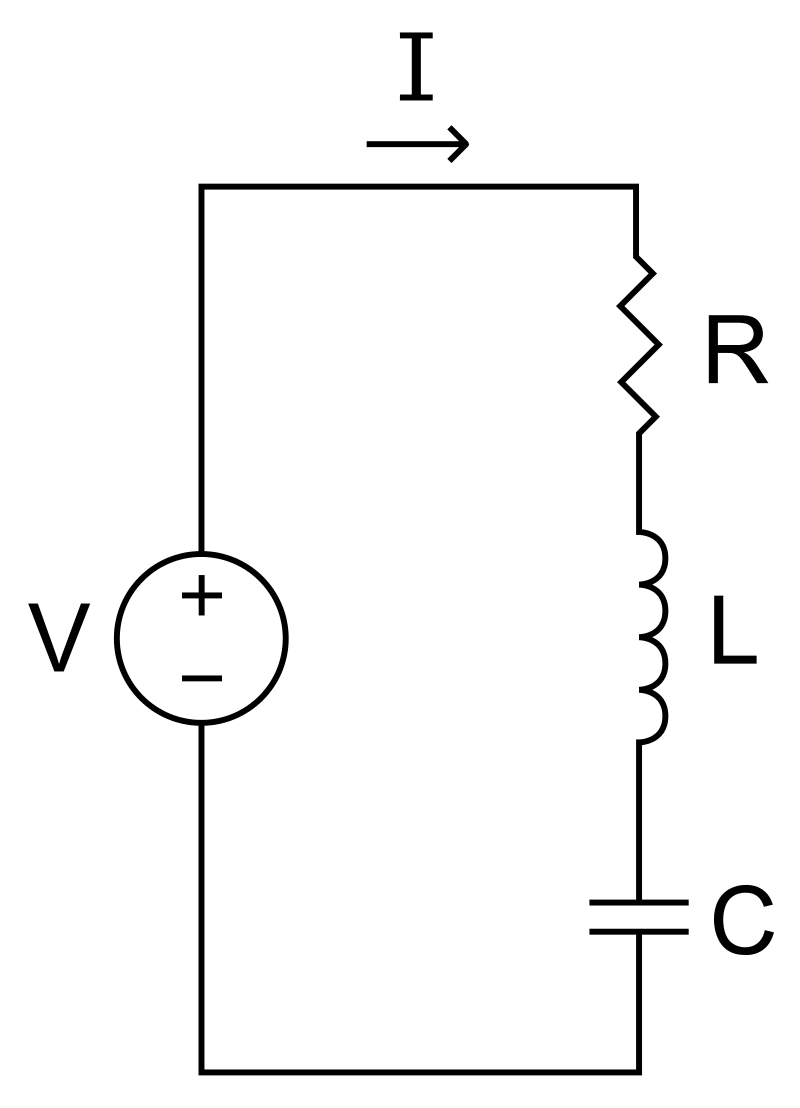
\includegraphics[width=0.33\textwidth]{s_r.png}
\caption{Serial Resonance Circuit}
\end{figure}
\subsection{阻抗特性}
$$\rho=\omega_0 L=\frac{1}{\omega_0 C}$$
\subsection{谐振频率} 
$$\omega_0=\frac{1}{\sqrt{LC}}$$
\begin{figure}[H]
\centering
\definecolor{qqqqff}{rgb}{0,0,1}
\definecolor{ccqqqq}{rgb}{0.8,0,0}
\definecolor{qqwuqq}{rgb}{0,0.39215686274509803,0}
\pgfplotsset{compat=1.15}
\begin{tikzpicture}
\begin{axis}[
% x=1cm,y=1cm,
axis lines=middle,
% ymajorgrids=true,
% xmajorgrids=true,
xmin=0,
xmax=6,
ymin=-2,
ymax=2,
ticks=none,
xtick={-1,-0.8,...,6.2},
ytick={-2.4000000000000004,-2.2,...,2},
xlabel={$\omega$},
ylabel={$X$电抗},
][
\clip(-1.190037014540084,-2.5059219515192663) rectangle (6.301753720696762,2.1789181652383323);
\draw[color=qqwuqq,smooth,samples=100,domain=-1.190037014540084:6.301753720696762] plot(\x,{(\x)/2});
\draw[color=ccqqqq,smooth,samples=100,domain=-1.190037014540084:6.301753720696762] plot(\x,{0-2/(\x)});
\draw[color=qqqqff,smooth,samples=100,domain=-1.190037014540084:6.301753720696762] plot(\x,{(\x)/2-2/(\x)});
\draw [dotted] (2,-2.5059219515192663) -- (2,2.1789181652383323);
\begin{scriptsize}
\draw[color=qqwuqq] (1,1) node {$\omega L$};
\draw[color=ccqqqq] (3,-1) node[right] {$-\frac{1}{\omega C}$};
\draw[color=qqqqff] (3,1) node[right] {$\omega L-\frac{1}{\omega C}$};
\draw[color=black] (2,0) node[below] {$\omega_0$};

\draw[color=qqqqff] (0,-1) node[right] {容性};
\draw[color=qqqqff] (3,0.5) node[right] {感性};
\end{scriptsize}
\end{axis}
\end{tikzpicture}
\caption{串联谐振回路--阻抗性质随频率变化的规律}
\end{figure}
$\omega>\omega_0$时呈容性\\
$\omega<\omega_0$时呈感性\\
当$\omega=\omega_0$时, $|\mathbb{Z}|=\sqrt{R^2+X^2}$最小, 此时$I$最大. 
$$\mathbb{Z}=R+j\cdot(\omega L-\frac{1}{\omega C})$$
谐振时, 电抗和为0, 即$\omega_0 L=\frac{1}{\omega_0 C}$
\subsection{品质因数}
$$Q_\text{serial}=\frac{X}{R}$$
\begin{figure}[H]
  \centering
  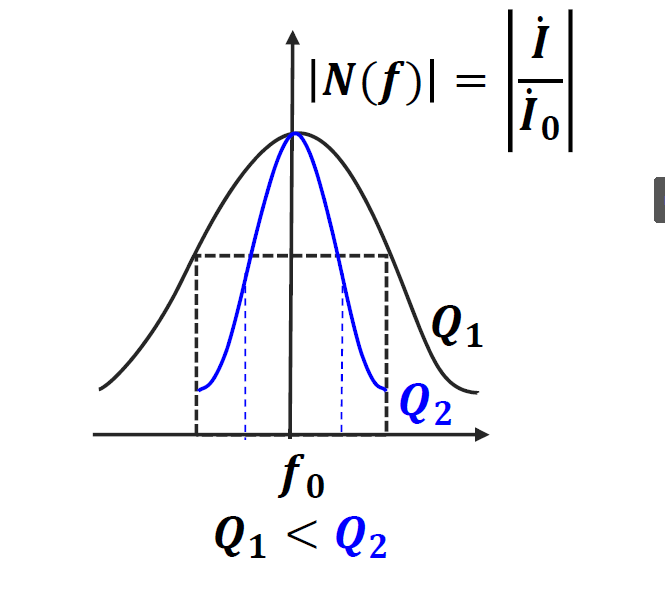
\includegraphics[width=0.6\textwidth]{s_r_graph.png}
  \caption{幅频特性曲线}
  \end{figure}
$$Q=\frac{\omega_0 L}{R}=\frac{1}{\omega_0 R C}$$
Q值越大, 曲线越尖锐, 选频作用越显著, 回路的选择性就越好. 
\subsection{通频带}
通频带又被称作$3dB$带宽. 以$2\Delta f_{0.7}$或者$B_{3dB}$表示. 
$$\text{Bandwith}=\frac{f_0}{Q_0}$$
\subsection{广义失谐系数$\xi$}
定义式
\begin{align*}
  Q_0&=\frac{X_C}{R}=\frac{X_L}{R}=\frac{\omega_0 L}{R}=\frac{1}{\omega_0 R C}\\
  \xi&=\frac{X}{R}=\frac{\omega L-\frac{1}{\omega C}}{R}
\end{align*}
计算式
$$\xi=Q_0\cdot\frac{2\Delta\omega}{\omega_0}=Q_0\cdot\frac{2\Delta f}{f_0}$$ 
\sout{$\Delta \omega,\Delta f$分别表示失谐时偏移的角速度(频率)的大小} \\\footnote{$\Delta\omega=|\omega-\omega_0|$, $\Delta f$同理}.\\
$2\Delta f$指的就是通频带$2\Delta f_{0.7}$, 即3dB带宽, 不是随随便便的频率偏移. 
\subsection{相频特性曲线}
$$\psi=-\arctan(\xi)$$
\begin{figure}[H]
\centering

\begin{tikzpicture}
  \begin{axis}[
      %domain=-10:10,
      xscale=1,yscale=1,
      xmin=-1.5, xmax=1.5,
      ymin=-2, ymax= 2,
      ticks=none,
      samples=1000,
      axis lines=center,
      ylabel={$\psi$},
      xlabel={$\omega$},
  ]
      %pos参数表示标签的位置(曲线从开始到结尾的) (分数)
      \addplot[smooth] {rad(-atan(x))} node[below,pos=.6]{$Q_1$};
      \addplot[color=blue,smooth] {rad(-atan(5*x))} node[above,pos=.4]{$Q_2$};
      %在pgfplot坐标系中需要用(axis cs:x,y)
      %可以使用textcolor给文字着色
      \draw (axis cs:1,1) node[above]{\textcolor{blue}{$Q_2>$} $Q_1$};
      %确实有above right
      \draw (axis cs:0,0) node[above right]{$\omega_0$};
  \end{axis}
\end{tikzpicture} 
\caption{串联谐振回路的相频特性曲线}
\end{figure}
Q值越大, 谐振频率$\omega_0$附近变化越陡峭. 线性度变差, 线性范围变窄. 
\subsection{有载Q值}
\begin{align*}
  Q_0&=\frac{\omega_0 L}{R}&&\text{空载Q值}\\
  Q_L&=\frac{\omega_0 L}{R+R_s+R_\text{Load}}&&\text{有载Q值, $R_s,R_L$分别为信号源的内阻和负载电阻}
\end{align*}
$R$为电感内阻. \\
$Q_L$降低, 通频带加宽. 
\section{Parallel}
\begin{figure}[H]
\centering
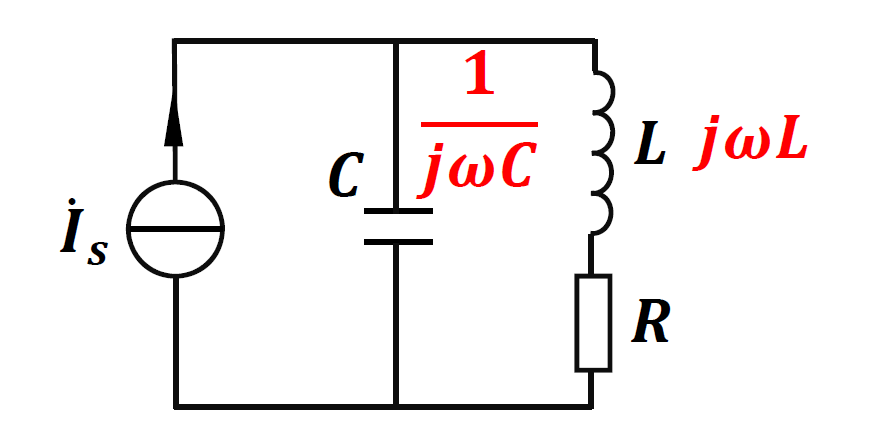
\includegraphics[width=0.33\textwidth]{p_r_1.png}
\caption{Parallel Resonance}
\end{figure}
\subsection{等效电阻}
\begin{figure}[H]
\centering
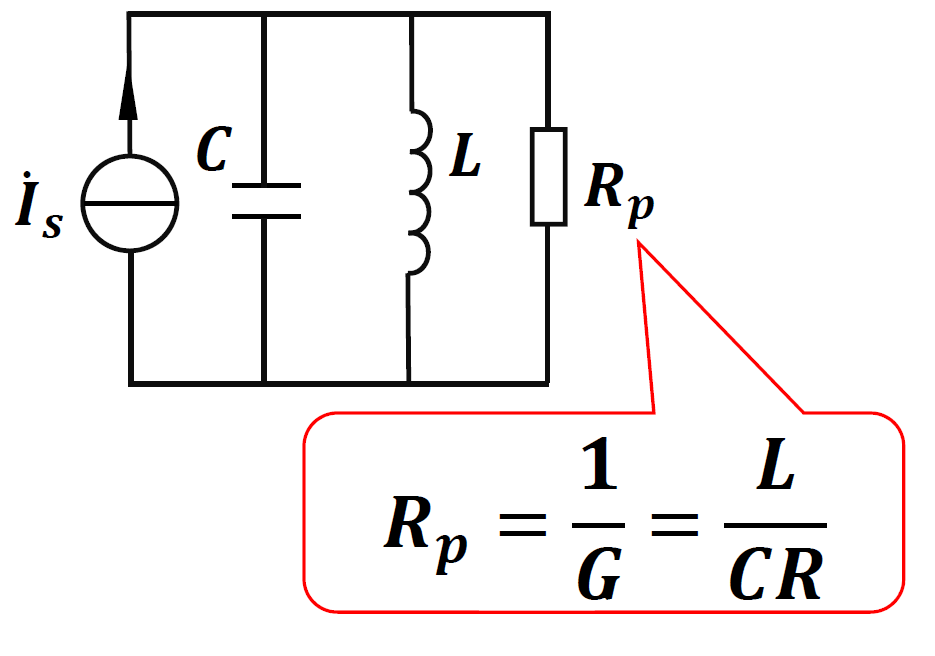
\includegraphics[width=0.33\textwidth]{p_r_2.png}
\caption{等效阻抗}
\end{figure}
原模型为电感串联电感的内阻$R$, 计算不变, 需要转换为三个元件并联的等效电阻. 
$$R_p=\frac{L}{RC}$$
总导纳
$$Y=G+jB=\frac{RC}{L}+j(\omega C-\frac{1}{\omega L})$$
\begin{figure}[H]
  \centering
  \definecolor{qqqqff}{rgb}{0,0,1}
  \definecolor{ccqqqq}{rgb}{0.8,0,0}
  \definecolor{qqwuqq}{rgb}{0,0.39215686274509803,0}
  \pgfplotsset{compat=1.15}
  \begin{tikzpicture}
  \begin{axis}[
  % x=1cm,y=1cm,
  axis lines=middle,
  % ymajorgrids=true,
  % xmajorgrids=true,
  xmin=0,
  xmax=6,
  ymin=-2,
  ymax=2,
  ticks=none,
  xtick={-1,-0.8,...,6.2},
  ytick={-2.4000000000000004,-2.2,...,2},
  xlabel={$\omega$},
  ylabel={$B$电纳},
  ][
  \clip(-1.190037014540084,-2.5059219515192663) rectangle (6.301753720696762,2.1789181652383323);
  \draw[color=ccqqqq,smooth,samples=100,domain=-1.190037014540084:6.301753720696762] plot(\x,{(\x)/2});
  \draw[color=qqwuqq ,smooth,samples=100,domain=-1.190037014540084:6.301753720696762] plot(\x,{0-2/(\x)});
  \draw[color=qqqqff,smooth,samples=100,domain=-1.190037014540084:6.301753720696762] plot(\x,{(\x)/2-2/(\x)});
  \draw [dotted] (2,-2.5059219515192663) -- (2,2.1789181652383323);
  \begin{scriptsize}
  \draw[color=ccqqqq] (1,1) node {$\omega C$};
  \draw[color=qqwuqq] (3,-1) node[right] {$-\frac{1}{\omega L}$};
  \draw[color=qqqqff] (3,1) node[right] {$\omega C-\frac{1}{\omega L}$};
  \draw[color=black] (2,0) node[below] {$\omega_p$};
  
  \draw[color=qqqqff] (0,-1) node[right] {感性};
  \draw[color=qqqqff] (3,0.5) node[right] {容性};
  \end{scriptsize}
  \end{axis}
  \end{tikzpicture}
  \caption{并联谐振回路--导纳性质随频率变化的规律}
  \end{figure}
  $$B=\omega C-\frac{1}{\omega L}$$
$\omega>\omega_0$时呈感性\\
$\omega<\omega_0$时呈容性\footnote{就是电容和电阻的表达式因为电纳而颠倒了过来}\\
当$\omega=\omega_0$时, $|\mathbb{Y}|=\sqrt{R^2+B^2}$最小\footnote{导纳最小}, 此时$I$最小. 
\subsection{谐振频率}
$$\omega_p=\frac{1}{\sqrt{LC}}$$
\subsection{品质因数}
\begin{align*}
  Q_\text{parallel}&=\frac{B}{G}\\
  Q_p&=\frac{1}{\omega_p L}\cdot R_p=\omega_p C\cdot R_p\\
  Q_p&=\frac{\frac{1}{\omega_p L}}{G}=\frac{\omega_p C}{G}=\frac{B}{G}&& R_p=\frac{1}{G}=\frac{L}{CR}
\end{align*}
\subsection{广义失谐系数}
$$\xi=\frac{\omega C-\frac{1}{\omega L}}{G}$$
\begin{align*}
  \xi=Q_p\cdot\frac{2\Delta f}{f_p}
\end{align*}
$2\Delta f$表示通频带. 
\begin{figure}[H]
  \centering
  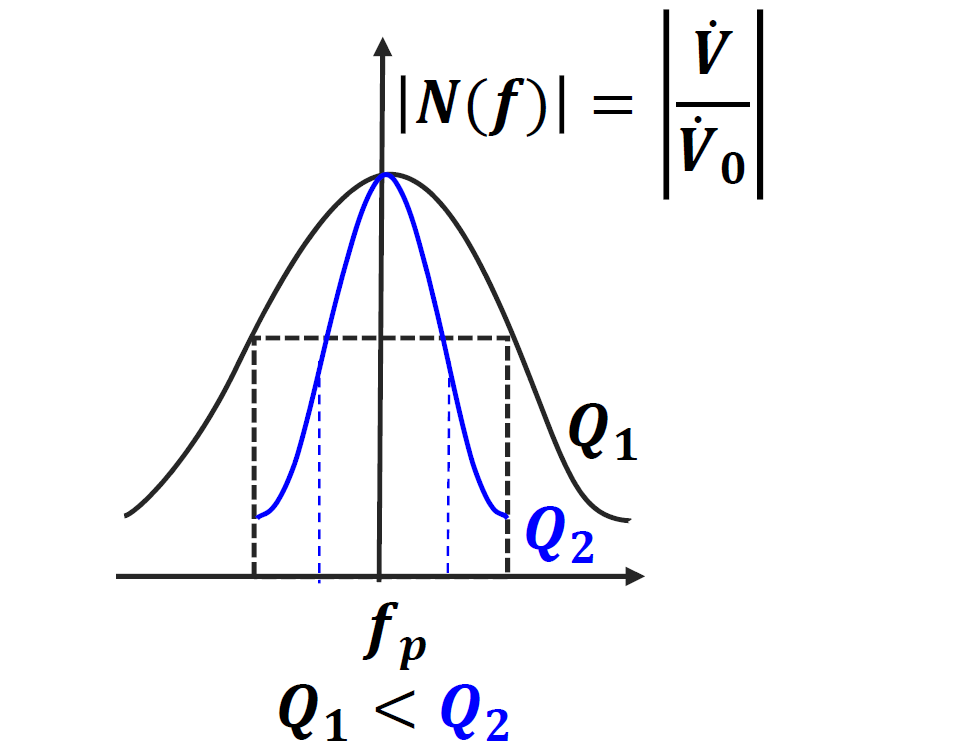
\includegraphics[width=0.6\textwidth]{p_r_graph.png}
  \caption{幅频特性曲线}
  \end{figure}
和串联谐振回路一样, Q值越大选择性越好. 
\subsection{相频特性曲线}
\label{sec:omega_phi_graph}
$$\psi=-\arctan(\xi)$$
\begin{figure}[H]
\centering

\begin{tikzpicture}
  \begin{axis}[
      %domain=-10:10,
      xscale=1,yscale=1,
      xmin=-1.5, xmax=1.5,
      ymin=-2, ymax= 2,
      ticks=none,
      samples=1000,
      axis lines=center,
      ylabel={$\psi$},
      xlabel={$\omega$},
  ]
      %pos参数表示标签的位置(曲线从开始到结尾的) (分数)
      \addplot[smooth] {rad(-atan(x))} node[below,pos=.6]{$Q_1$};
      \addplot[color=blue,smooth] {rad(-atan(5*x))} node[above,pos=.4]{$Q_2$};
      %在pgfplot坐标系中需要用(axis cs:x,y)
      %可以使用textcolor给文字着色
      \draw (axis cs:1,1) node[above]{\textcolor{blue}{$Q_2>$} $Q_1$};
      %确实有above right
      \draw (axis cs:0,0) node[above right]{$\omega_0$};
  \end{axis}
\end{tikzpicture} 

\caption{并联谐振回路的相频特性曲线}
\end{figure}
Q值越大, 谐振频率$\omega_0$附近变化越陡峭. 线性度变差, 线性范围变窄. \footnote{看着眼熟么? 就是从上一节直接复制过来的, 和串联谐振回路一模一样}
\subsection{有载Q值}
\begin{align*}
  Q_p&=\frac{1}{\omega_p L}\cdot R_p=\frac{1}{\omega_p L\cdot G} &&G_p=\frac{1}{R_p}=\frac{CR}{L}\\
  Q_L&=\frac{1}{\omega_p L}\cdot \frac{1}{G_p+G_s+G_\text{Load}}
\end{align*}
$G_s,G_L$分别为内阻和负载的电导\\
$Q_L$降低, 通频带加宽. 
\subsection{小结}
\begin{figure}[H]
\centering
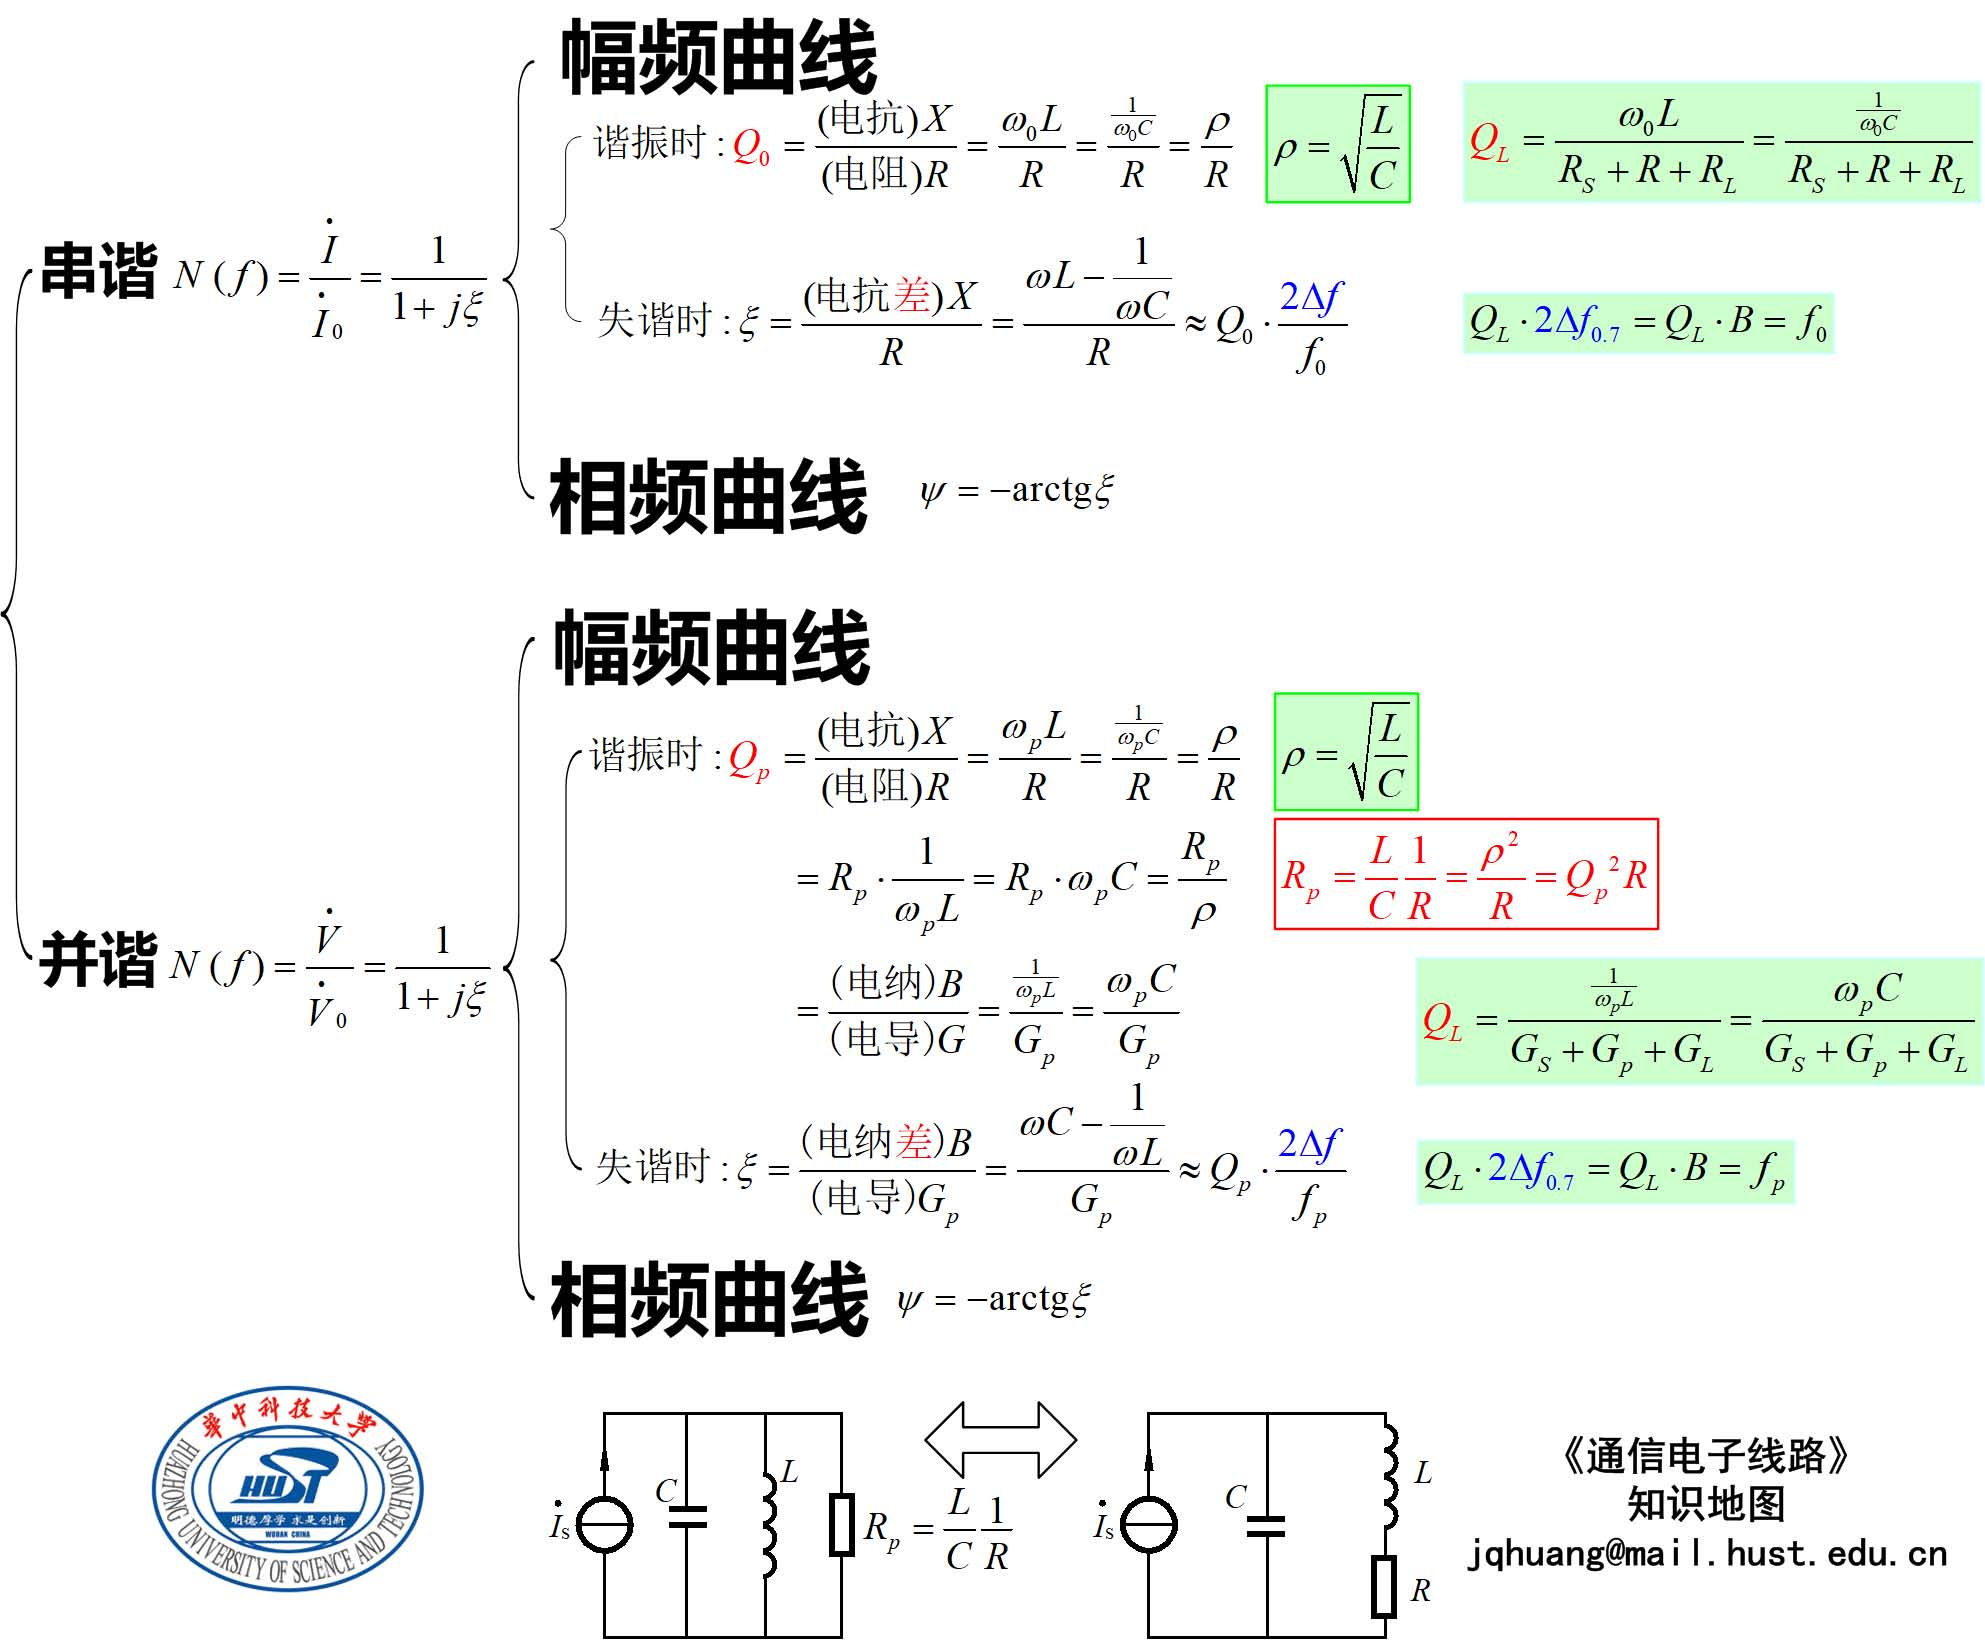
\includegraphics[width=1\textwidth]{res_map.jpg}
\caption{知识地图}
\end{figure}
\section{阻抗变换}
\begin{figure}[H]
\centering
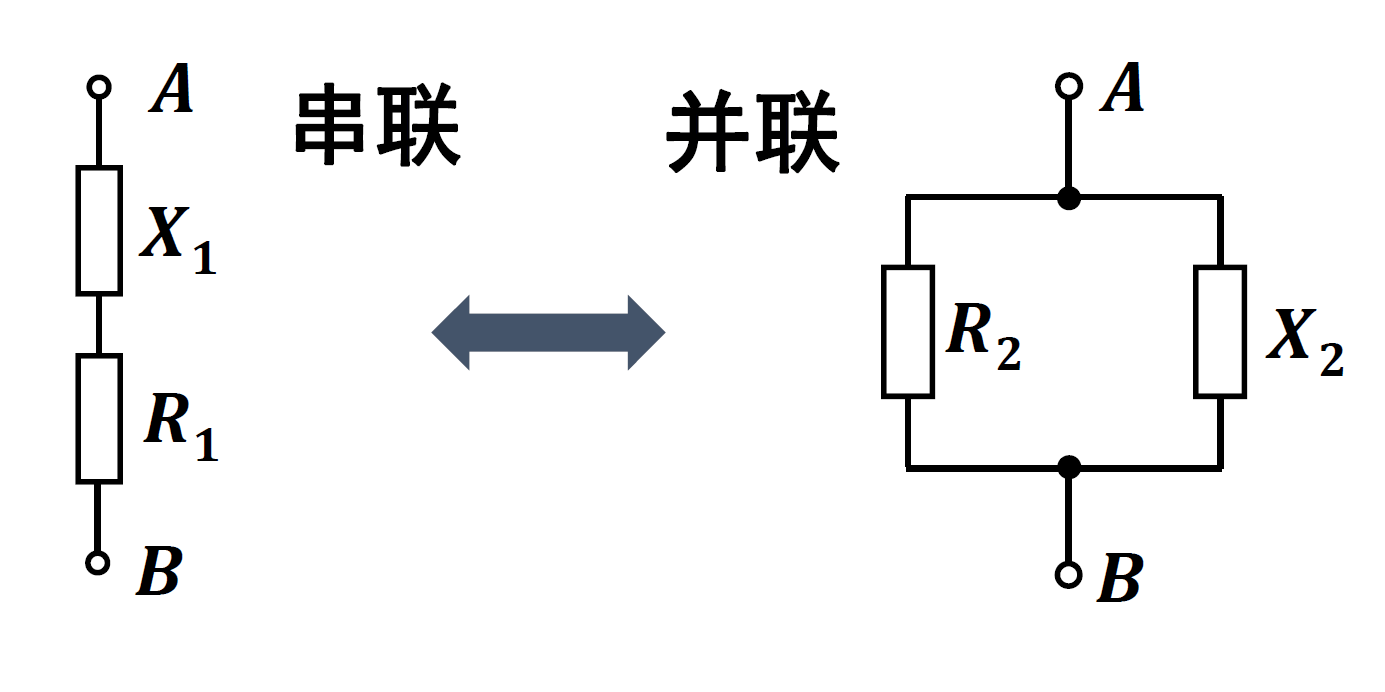
\includegraphics[width=0.6\textwidth]{s_r_conversion.png}
\caption{阻抗变换}
\end{figure}
\subsection{阻抗相等}
$$
  \begin{cases}
    R_s=\frac{R_p\cdot X_p^2}{R_p^2+X_p^2}\\
    X_s=\frac{R_p^2\cdot X_p}{R_p^2+X_p^2}
  \end{cases}
  \begin{cases}
    R_p=R_s\cdot(1+Q^2)\\
    X_p=X_s\cdot(1+\frac{1}{Q^2})
  \end{cases}
$$

当Q值较高(大于10时)
\begin{align*}
  R_p\approx R_s\cdot Q^2\\
  X_p\approx X_s
\end{align*}

\begin{itemize}
  \item 电阻:串联时远小于并联(小的$R_s$变成大的$R_p$)
  \item 电抗: 串联或者并联时大小/性质不变 ($X_p$与$X_s$性质相同, 大小相等)
\end{itemize}

\subsection{Q相等} 
$$Q=\frac{X_s}{R_s}=\frac{R_p}{X_p}$$

\section{抽头(部分接入)}
\subsection{电感抽头}
\begin{figure}[H]
\centering
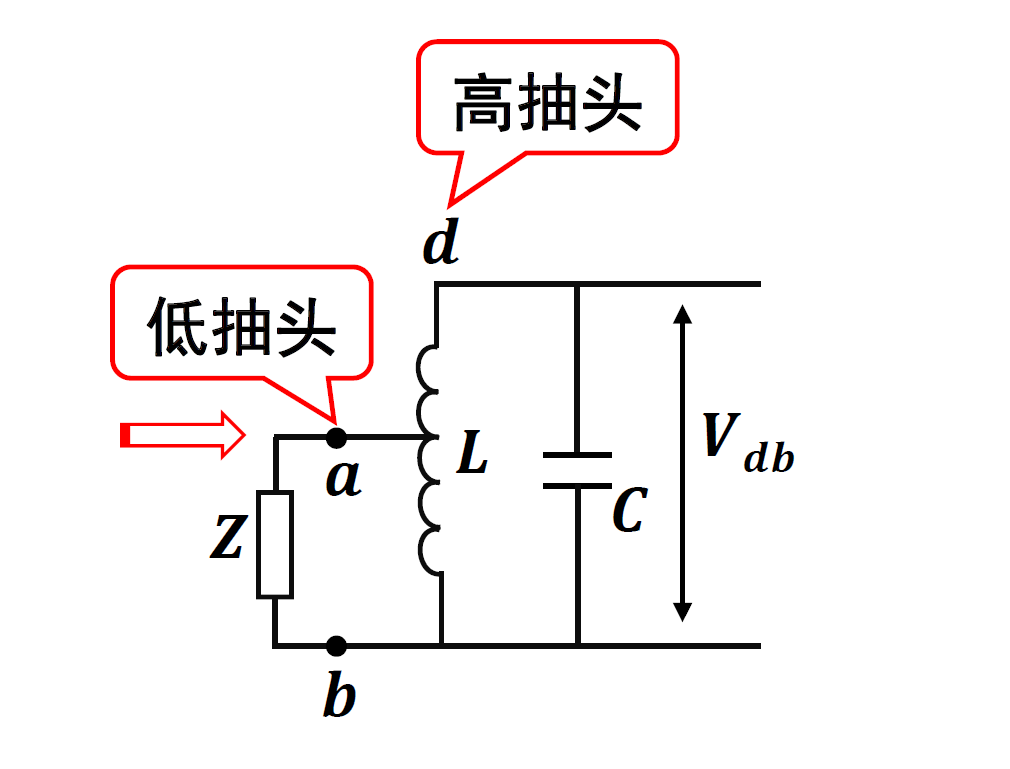
\includegraphics[width=0.4\textwidth]{tap_l.png}
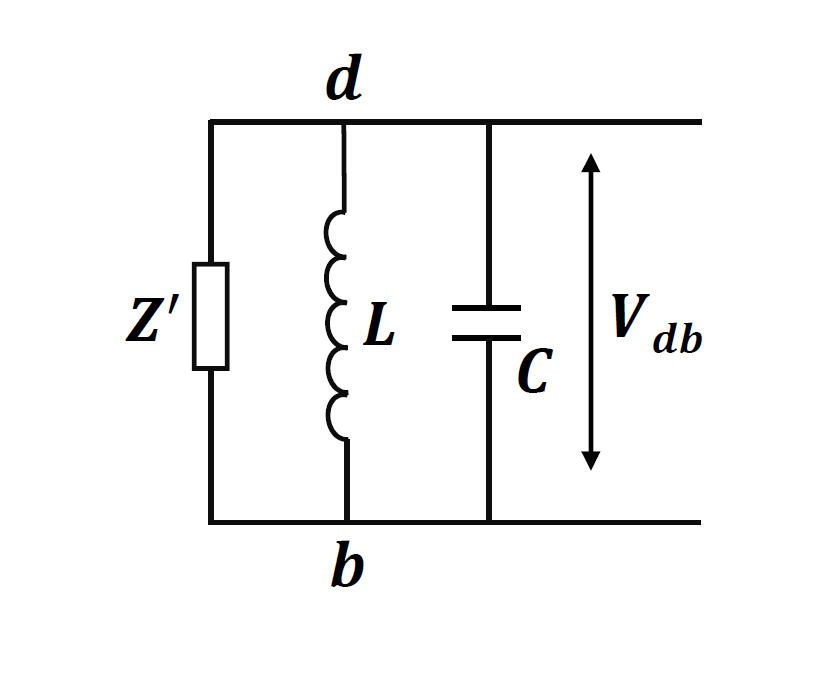
\includegraphics[width=0.4\textwidth]{tap_l_equ.png}
\caption{电感抽头电路及其等效电路}
\end{figure}
接入系数
\begin{align*}
  p&=\frac{L_{ab}}{L_{db}}=\frac{ L_{\text{接入的那段}} }{ L_\text{整条电感} }\\
   &=\frac{ L_{\text{接入的那段}}\pm \text{互感} }{ L_\text{整条电感}\pm \text{两倍的互感} }&&有互感情况时\\
   &=\frac{L_{ab}\pm M}{L_{db}\pm 2M}&&有互感情况时\\
   &=\frac{N_{\text{接入的那段}}}{N_{\text{整条电感}}}
\end{align*}
通常$p<1$, 即低抽头向高抽头转\footnote{以prime表示高抽头, 无上下标表示低抽头}时, 等效阻抗提高$\frac{1}{p^2}$. 
\begin{align*}
  Z'&=\frac{1}{p^2}\cdot Z\\
  Y'&=p^2\cdot Y\\
  V'&=\frac{1}{p}\cdot V\\
  I'&=p\cdot I
\end{align*}
抽头前后功率等效
\begin{align*}
  P'&=P\\
  V'\cdot I'&=V\cdot I
\end{align*}
\subsubsection{低抽头到高抽头}
常见于信号源的部分接入
\subsubsection{高抽头到低抽头}
常见于负载的部分接入
\subsection{电容抽头}
\begin{figure}[H]
\centering
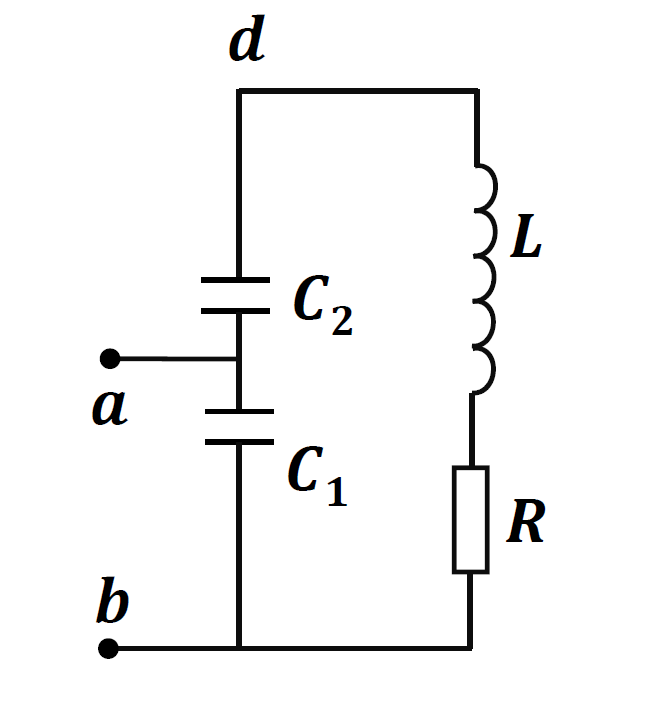
\includegraphics[width=0.33\textwidth]{tap_c.png}
\caption{电容抽头}
\end{figure}
接入系数
\begin{align*}
  p&=\frac{C_{\text{串联电容值}}}{C_{\text{接入的那部分}}}\\
  &=\frac{\frac{C_1\cdot C_2}{C_1+C_2}}{C_1}\\
  &=\frac{C_2}{C_1+C_2}\\
  &=\frac{C_{\text{没接入那部分}}}{C_{\text{并联电容值}}}\\
  &=\frac{C_{\text{没接入那部分}}}{\text{两电容值之和}}
\end{align*}
其他同上一小节. 
\section{耦合回路}
耦合系数 (coupling coefficient)$k$, $M$为互感, $L$为电感值 \\
耦合因数 (coupling factor)$\eta$
\begin{align*}
  k&=\frac{M}{\sqrt{L_1\cdot L_2}}\\
  \eta&=Q\cdot k
\end{align*}
\begin{itemize}
  \item $\eta<1$ 为欠耦合 (under coupling)
  \item $\eta=1$ 为临界耦合 (critical coupling)
  \item $\eta>1$ 为过耦合 (over coupling) 
\end{itemize}
\section{石英晶体滤波器}
石英晶体具有压电效应 (piezoelectric effect)\\
正压电效应, 受机械力, 晶体表面产生电荷\\
反压电效应, 外加电压, 晶体产生机械震动 (振动大小基本正比于外加电压幅度)
\begin{figure}[H]
\centering
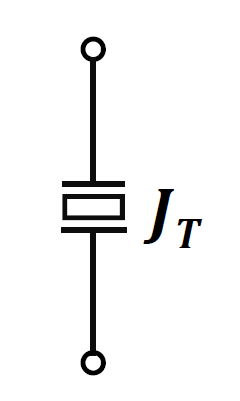
\includegraphics[width=0.1\textwidth]{crystal_2.png}
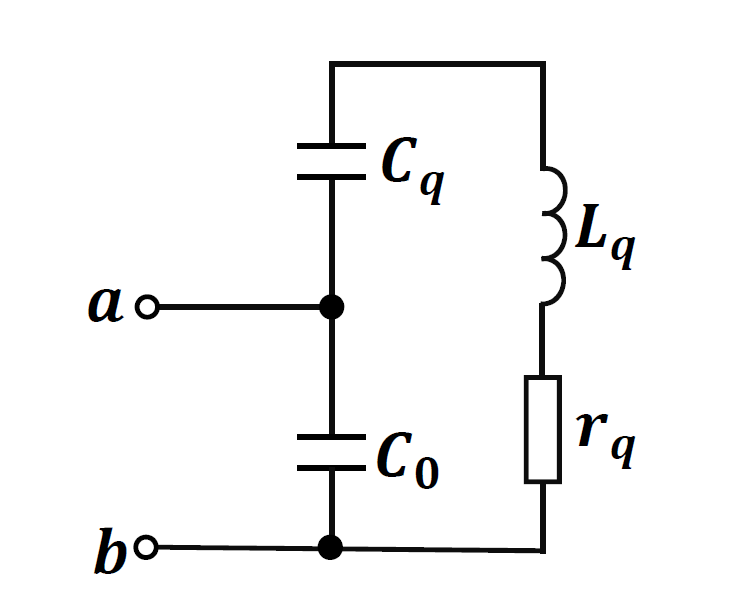
\includegraphics[width=0.5\textwidth]{crystal_1.png}
\caption{石英晶体振荡器及其等效电路}
\end{figure}
\begin{align*}
  \omega_q=\omega_{\text{serial}}=\frac{1}{\sqrt{L_q C_q}}\\
  \omega_p=\omega_{\text{parallel}}=\frac{1}{\sqrt{L_q\cdot\frac{C_0 C_q}{C_0+C_q}}}
\end{align*}

\begin{itemize}
  \item 接入系数p很小
  \item Q值$\frac{1}{r_q}\cdot\sqrt{\frac{L_q}{C_q}}$很大
\end{itemize}
\subsection{电抗频率曲线}
\begin{figure}[H]
\centering
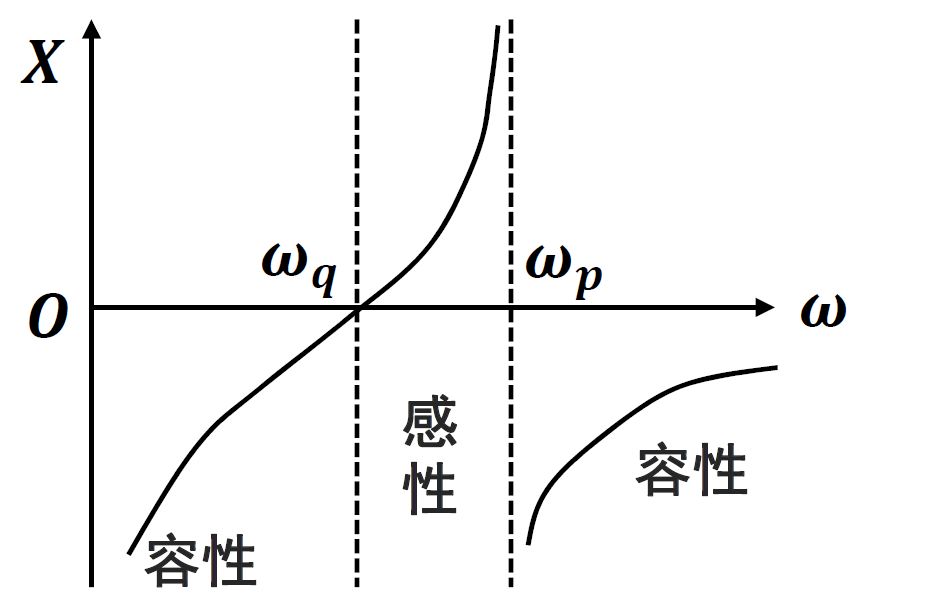
\includegraphics[width=0.5\textwidth]{crystal_graph.png}
\caption{电抗频率曲线}
\end{figure}
感性区其实很小. 为了增大感性区可以采取
\begin{itemize}
  \item 串联电感以减小串联频率
  \item 并联电容以增大并联频率
\end{itemize}

\chapter{高频小信号放大器}
高频放大器与低频(音频)放大器的主要区别在于两者的工作频率范围和所需通过频带宽度都有所不同. \\
高频放大器与低频放大器比较
\begin{itemize}
  \item 低频工作频率低, 高频工作频率高
  \item 低频工作频带宽度宽, 高频通频带窄 (窄带)
\end{itemize}
高频谐振小信号放大器用于接收端. 俗称小放. 信号高频谐振放大器用来对高频小信号进行选频和放大. 
\begin{itemize}
  \item 负载采用LC 谐振回路,放大器具有选频作用,为窄带放大器。
  \item 有较高的增益,适用于窄带信号的放大。
  \item 放大器工作在甲类线性工作状态,可采用高频小信号等效电路进行分析。
\end{itemize}
\begin{quotation}
  \centering
  放大器+选频网络 \footnote{采用谐振回路作为负载的放大器, 被称作谐振放大器 (resonant amplifier)}
\end{quotation}
\section{质量指标}
\begin{itemize}
  \item 增益 (gain)
  \item 通频带 (passband)
  \item 选择性 (selectivity)
  \begin{itemize}
    \item 矩形系数 rectangular coefficient
    \item 抑制比 suppression ratio
  \end{itemize}
  \item 稳定性 (stability)
  \item 噪声系数 (noise figure)
\end{itemize}
\subsection{增益}
电压增益
$$\mathbb{A}_V=\frac{\mathbb{V}_o}{\mathbb{V}_i}$$
\subsubsection{电压增益与频率曲线}
\begin{figure}[H]
\centering
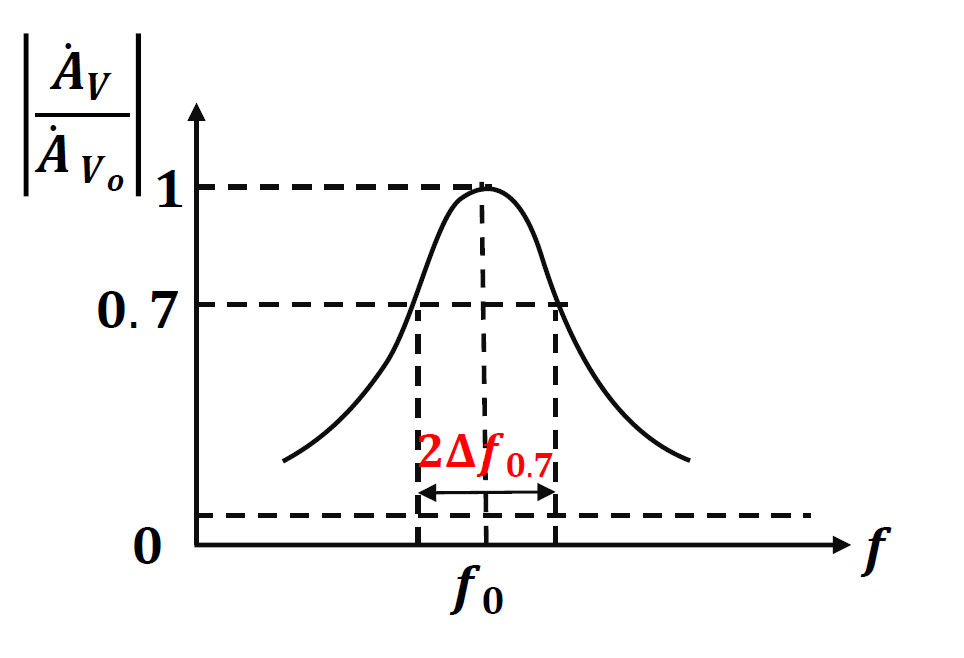
\includegraphics[width=0.5\textwidth]{amp_small_graph_1.png}
\caption{电压增益与频率幅度曲线}
\end{figure}
$\mathbb{A}_V$是一个关于频率$f$的函数, $\mathbb{A}_{V0}$则是谐振频率时的增益
$$|\frac{\mathbb{A}_V}{\mathbb{A}_{V_0}}(f)|=\frac{1}{\sqrt{2}}\approx 0.707\Rightarrow 2\Delta f_{0.7}$$

\subsection{选择性}
\subsubsection{矩形系数}
\begin{figure}[H]
\centering
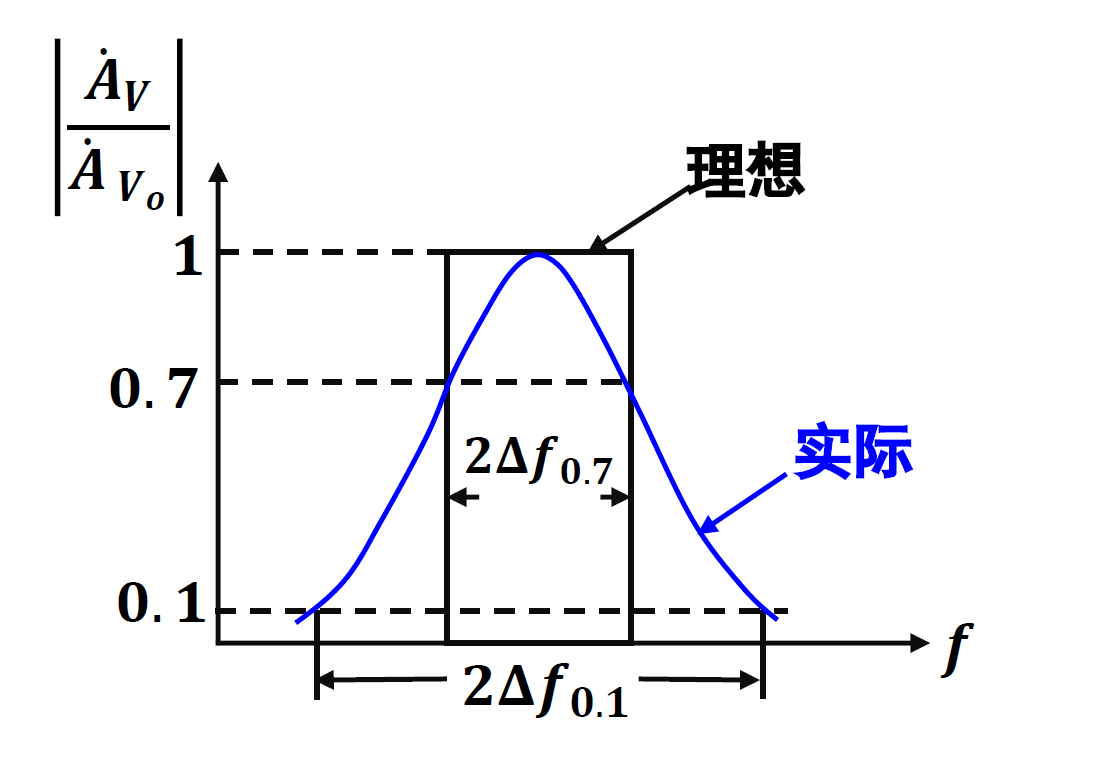
\includegraphics[width=0.33\textwidth]{amp_small_graph_2.png}
\caption{矩形系数}
\end{figure}
表示曲线接近理想曲线的程度
$$K_{r0.1}=\frac{2\Delta f_{0.7}}{2\Delta f_{0.1}}$$
怎么得到$2\Delta f_{0.1}$呢? 求出增益$\mathbb{A}_V(f)$关于频率的函数表达式, RHS等于0.1, 解出频率即可. 
\subsubsection{抑制比}
\begin{figure}[H]
\centering
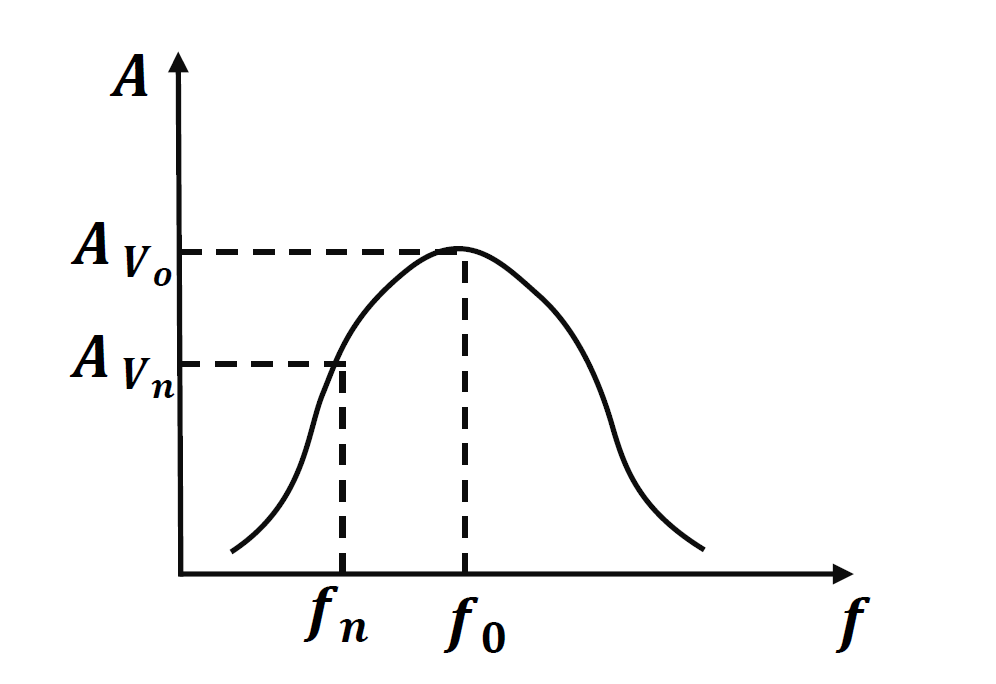
\includegraphics[width=0.33\textwidth]{amp_small_graph_3.png}
\caption{抑制比}
\end{figure}
表示对某干扰信号$f_n$的抑制能力. 
$$d_n=\frac{A_{V_0}}{A_{V_n}}$$
如何得到$A_{V_n}$? 求出增益$\mathbb{A}_V(f)$关于频率的函数表达式, 把$f_n$代进去就好了. 
\subsection{稳定性}
自激
\subsection{噪声系数}
$$\text{SNR}=\frac{\text{Signal}}{\text{Noise}}$$
$$N_F=\frac{\text{SNR}_{\text{input}}}{\text{SNR}_{\text{output}}}$$
噪声系数越接近1越好. 
\section{晶体管的高频参数}
共射电路的电流放大系数$\beta$会随着工作频率的上升而下降
$$f_\text{max}>f_T>f_\beta$$
\subsection{截止频率}
cut-off frequency $f_\beta$\\
当$\beta$下降到低频$\beta_0$的$\frac{1}{\sqrt{2}}$时的频率. \\
晶体管仍然可以起到放大作用
\subsection{特征频率}
characteristic frequency $f_T$\\
当频率升高使得晶体管的$\beta$下降到1时的频率\\
当$\beta_0\gg 1$时
$$f_T\approx \beta_0\cdot f_\beta$$
\subsection{最高震荡频率}
$f_\text{max}$晶体管所能适用的最高极限频率. \\
一般实际工作频率取最高振荡频率的$\frac{1}{4}\sim\frac{1}{3}$
\section{单极谐振小信号放大器}
高频谐振小信号放大器=晶体管+并联谐振回路 (抽头)
\subsection{Y参数等效模型}
\begin{figure}[H]
\centering
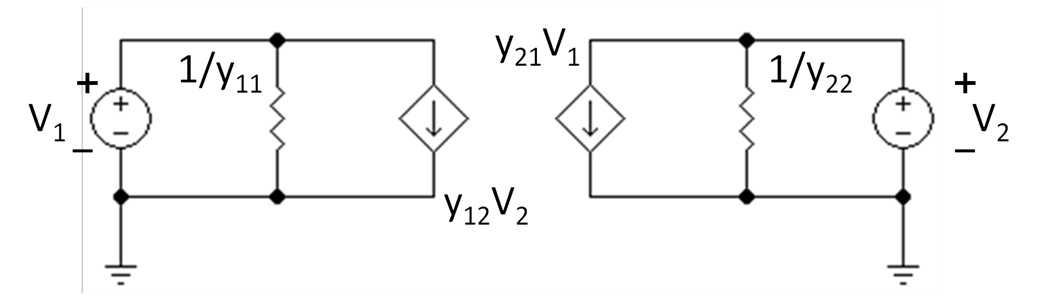
\includegraphics[width=0.5\textwidth]{y_para.png}
\caption{Y Parameter}
\end{figure}
题目直接给Y参数\footnote{Shunt admittance}
\begin{itemize}
  \item 输入导纳 $y_{ie}$ ($y_{11}$)
  \item 正向传输导纳 $y_{fe}$ ($y_{21}$)
  \item 反向传输导纳 $y_{re}$ ($y_{12}$)
  \item 输出导纳 $y_{oe}$ ($y_{22}$)
\end{itemize}
高频谐振小信号放大器=晶体管Y参数等效电路+并联谐振回路 (抽头)\\
注意加上$R_p$

$y$是个复数, 题目会给$g$和$C$
\begin{align*}
  Y&=G+jB\\
  Y&=G+j\omega C-j\cdot \frac{1}{\omega L}
\end{align*}
偏置电阻算在$y_{ie}$里面. 

出于分析的方便,假定晶体管不存在内反馈,即$y_{re}=0$\\
把晶体管集电极回路\footnote{假设下一级有晶体管的话\dots}和负载, 折合到振荡回路两端
\begin{figure}[H]
\centering
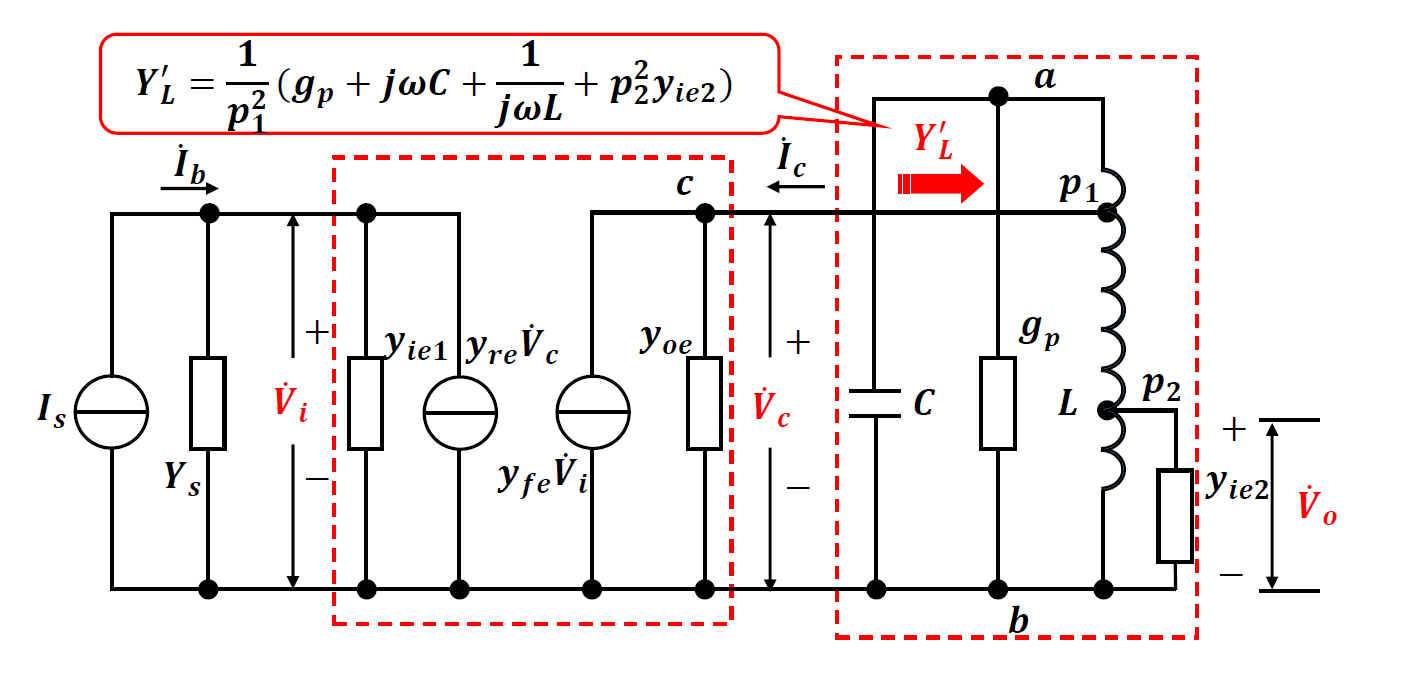
\includegraphics[width=0.8\textwidth]{amp_small_circuit_1.png}
\caption{高频小信号放大器等效电路图}
\end{figure}
\begin{align*}
  \mathbb{A}_V&=\frac{-p_1p_2\cdot |y_{fe}|}{Y_\Sigma}\\
  &=\frac{-p_1p_2\cdot |y_{fe}|}{g_\Sigma+j\cdot B_\Sigma}\\
  &=\frac{-p_1p_2\cdot |y_{fe}|}{g_\Sigma+j\omega C_\Sigma +\frac{1}{j\omega L}}
\end{align*}
当谐振时$j\omega C_\Sigma+\frac{1}{j\omega L}=0$, 即$j\cdot B=0$
$$\mathbb{A}_{V_0}=\frac{-p_1p_2y_{fe}}{g_\Sigma}$$
\subsection{计算方法}
一般题目会给条件
\begin{align*}
  y_{re}&=0\\
  y_{ie}&=g_{ie}+j\omega C_{ie}\\
  y_{oe}&=g_{oe}+j\omega C_{oe}\\
  |y_{fe}|&=\text{const}
\end{align*}
然后假设\textbf{上一级}, \textbf{下一级}所用的晶体管类型一样, 即$y$参数一样. \\
列等效模型时, 只需要列第一级晶体管的$y_{oe}$和$|y_{fe}|$, 不用理$y_{ie}$. 但同时需要计算下一级晶体管接入的$y_{ie}$. 如果把它们全部接入到谐振网络的话有
\begin{align*}
  g_{oe+ie}=p_1^2\cdot y_{oe1}+p_2^2\cdot y_{ie2}
\end{align*}
$p_1,p_2$分别为接入系数. $y_{oe1}$表示本级的输出导纳, $y_{ie2}$表示下一级的输入导纳 (或者可以说时负载导纳) 

具体接入方式如下图
\begin{figure}[H]
\centering
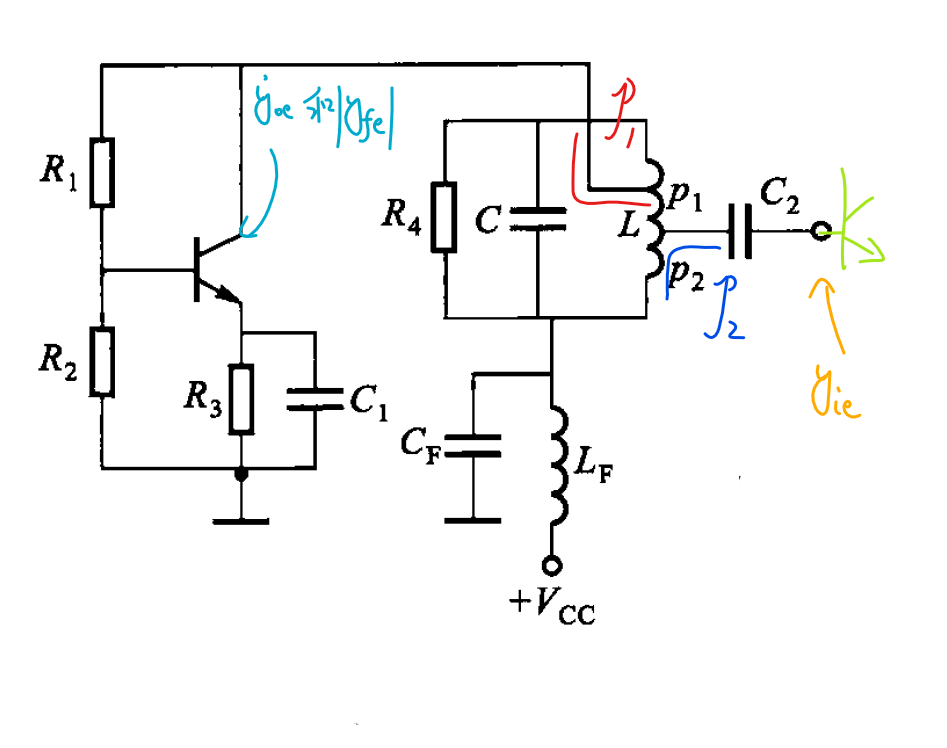
\includegraphics[width=0.5\textwidth]{amp_small_circuit_y.png}
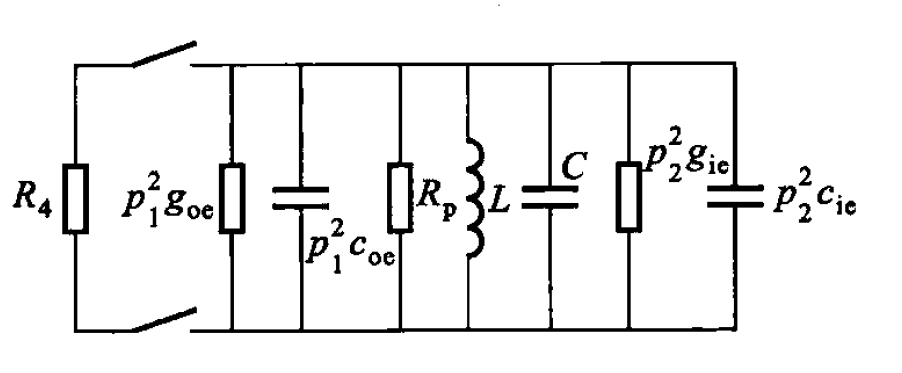
\includegraphics[width=0.5\textwidth]{amp_small_circuit_2.png}
\caption{接入方式}
\end{figure}
就是假设每一级都是这样的形式来计算的. 所以左边的晶体管只算$y_{oe}$, 右边的晶体管连着 \footnote{虽然没出现, 但假设连着的话}只算$y_{ie}$, 就十分简单了. 
\subsection{质量指标计算}
\subsubsection{电压增益}
\begin{align*}
  \mathbb{A}_{v0}&=-\frac{p_1p_2\cdot y_{fe}}{g_\Sigma}\\
  |\mathbb{A}_{v0}|_\text{max}&=\frac{|y_{fe}|}{2\sqrt{g_{o1}\cdot g_{i2}}}
\end{align*}
电压增益可以用分贝表示, 注意系数是20
\begin{align*}
  A_{\text{decibel V}}=20\cdot \log_{10}(A_{\text{linear V}})
\end{align*}
\subsubsection{功率增益}
只讨论谐振时的功率增益
\begin{align*}
  A_{p0}&=(A_{v0})^2\cdot \frac{g_{i2}}{g_{i1}} &&\text{$g_{i1},g_{i2}$分别为本级和下一级的输入电导}\\
  A_{p0}&=(A_{v0})^2 &&\text{当多级参数相同时}
\end{align*}
功率增益可以用分贝表示, 注意系数是10
\begin{align*}
  A_{\text{decibel P}}=10\cdot \log_{10}(A_{\text{linear P}})
\end{align*}
\subsubsection{通频带}
$Q_L$为有载Q值, $f_0$为谐振频率
\begin{align*}
  2\Delta f_{0.7}=\frac{f_0}{Q_L}
\end{align*}
总电容$C_\Sigma$愈大, 通频带$2\Delta f_{0.7}$愈宽, 增益$A_{v0}$愈小. 
\section{多级谐振小信号放大器}
单调谐放大器经过级联后电压增益\textbf{增大}、通频带\textbf{变窄}、选择性\textbf{变好}
\subsection{增益}
多级增益是单级增益之积
$$A_{\text{n级增益}}=A_1\cdot A_2\cdot A_3\dots \cdot A_n$$
若每极增益相同为$A$
$$A_{\text{n级增益}}=A^n$$
电压增益可以用分贝表示, 注意系数是20
\begin{align*}
  A_{\text{decibel V}}=20\cdot \log_{10}(A_{\text{linear V}})
\end{align*}
\subsection{通频带}
若每一级的增益相同. 单极通频带为$2\Delta f_{0.7}$
$$(2\Delta f_{0.7})_n=\sqrt{2^{\frac{1}{n}}-1}\cdot 2\Delta f_{0.7}$$
令系数$X=\sqrt{2^{\frac{1}{n}}-1}$为带宽缩减因子 (其值小于1). 
\begin{itemize}
  \item 总通频带$<$单极通频带
  \item 为了使总通频带不变, 每级通频带均要增加为原来的$\frac{1}{\text{带宽缩减因子}}$倍. 
  \item 但每级增益均会降低为原来的「带宽缩减因子」倍
\end{itemize}
\subsection{选择性}
$$(2\Delta f_{0.1})_n=\sqrt{100^{\frac{1}{n}}-1}\cdot 2\Delta f_{0.7}$$
$$K_{r0.1}=\frac{(2\Delta f_{0.1})_n}{(2\Delta f_{0.7})_n}=\frac{\sqrt{100^{\frac{1}{n}}-1}}{\sqrt{2^{\frac{1}{n}}-1}}$$
  % Table generated by Excel2LaTeX from sheet 'Sheet1'
  \begin{table}[H]
    \centering
    \caption{级别与矩形系数}
\resizebox{\textwidth}{!}{
      \begin{tabular}{cccccccccc}
      $n$级     & 1     & 2     & 3     & 4     & 5     & 6     & 7     & 8     & $\infty$ \\
      \hline
      $K_r$    & 9.949874 & 4.661322 & 3.743042 & 3.380547 & 3.188647 & 3.070322 & 2.990204 & 2.932412 & 2.56 \\
      \end{tabular}%
}
  \end{table}%


\section{双调谐回路放大器}
为了改善\textbf{选择性}和\textbf{增益与通频带的矛盾}, 可以采用双调谐回路放大器和参差调谐放大器.\\
在电路参数相同的情况下, 双调谐回路与单调谐回路相比. 

\begin{itemize}
  \item 通频带\textbf{增大} $2\Delta f_{0.7}=\sqrt{2}\cdot \frac{f_0}{Q_L}$
  \item 矩形系数更小, 更接近1 (即选择性更好)
\end{itemize}
\section{自激}
自激产生的原因是晶体管集电极电容的反馈作用, 由于反馈导纳$y_{re}$的存在, 改变了回路的等效品质因数$Q_L$, 引起回路的失谐.  
\subsection{稳定系数}
$S$稳定系数. 
\begin{itemize}
  \item $S=1$时产生自激
  \item $S\gg 1$(远大于) 时稳定, 放大器才能正常工作 (一般要求稳定系数为5至10)
\end{itemize}
当$S=5$时, 有稳定电压增益 $(A_{V_0})_S=\sqrt{\frac{|y_{fe}|}{2.5\omega_0 C_{re}}}$ 
稳定电压增益是保持放大器稳定工作所允许的电压增益. 
\begin{itemize}
  \item $(A_{V_0})_S$与频率$f$有关, 频率增大稳定电压增益减小
  \item 管子选$\frac{y_{fe}}{C_{re}}$大一些的好
  \item $(A_{V_0})_S$ 只考虑内部反馈, 未考虑外部反馈
\end{itemize}
\subsection{克服自激方法}
单向化 (消除$y_{re}$影响)
\subsubsection{中和法}
加外反馈抵消内反馈\\
在BJT的输出和输入端之间引入一个附加的外部反馈电路. 
\paragraph{优点}
\begin{itemize}
  \item 简单, 增益较高
\end{itemize}
\paragraph{缺点}
\begin{itemize}
  \item 调整麻烦
\end{itemize}
\subsubsection{失配法}
降低增益减少输出减少反馈. 使负载电导或者信号源电导的数值加大, 使得输入或者输入回路与BJT失去匹配. \\
典型电路时共射-共基级联放大器. \\
共基放大器的输入阻抗很低, 输出阻抗很高. 
\paragraph{优点}
\begin{itemize}
  \item 频带宽
\end{itemize}
\paragraph{缺点}
\begin{itemize}
  \item 增益较低
\end{itemize}
\section{小结}
\begin{figure}
\centering
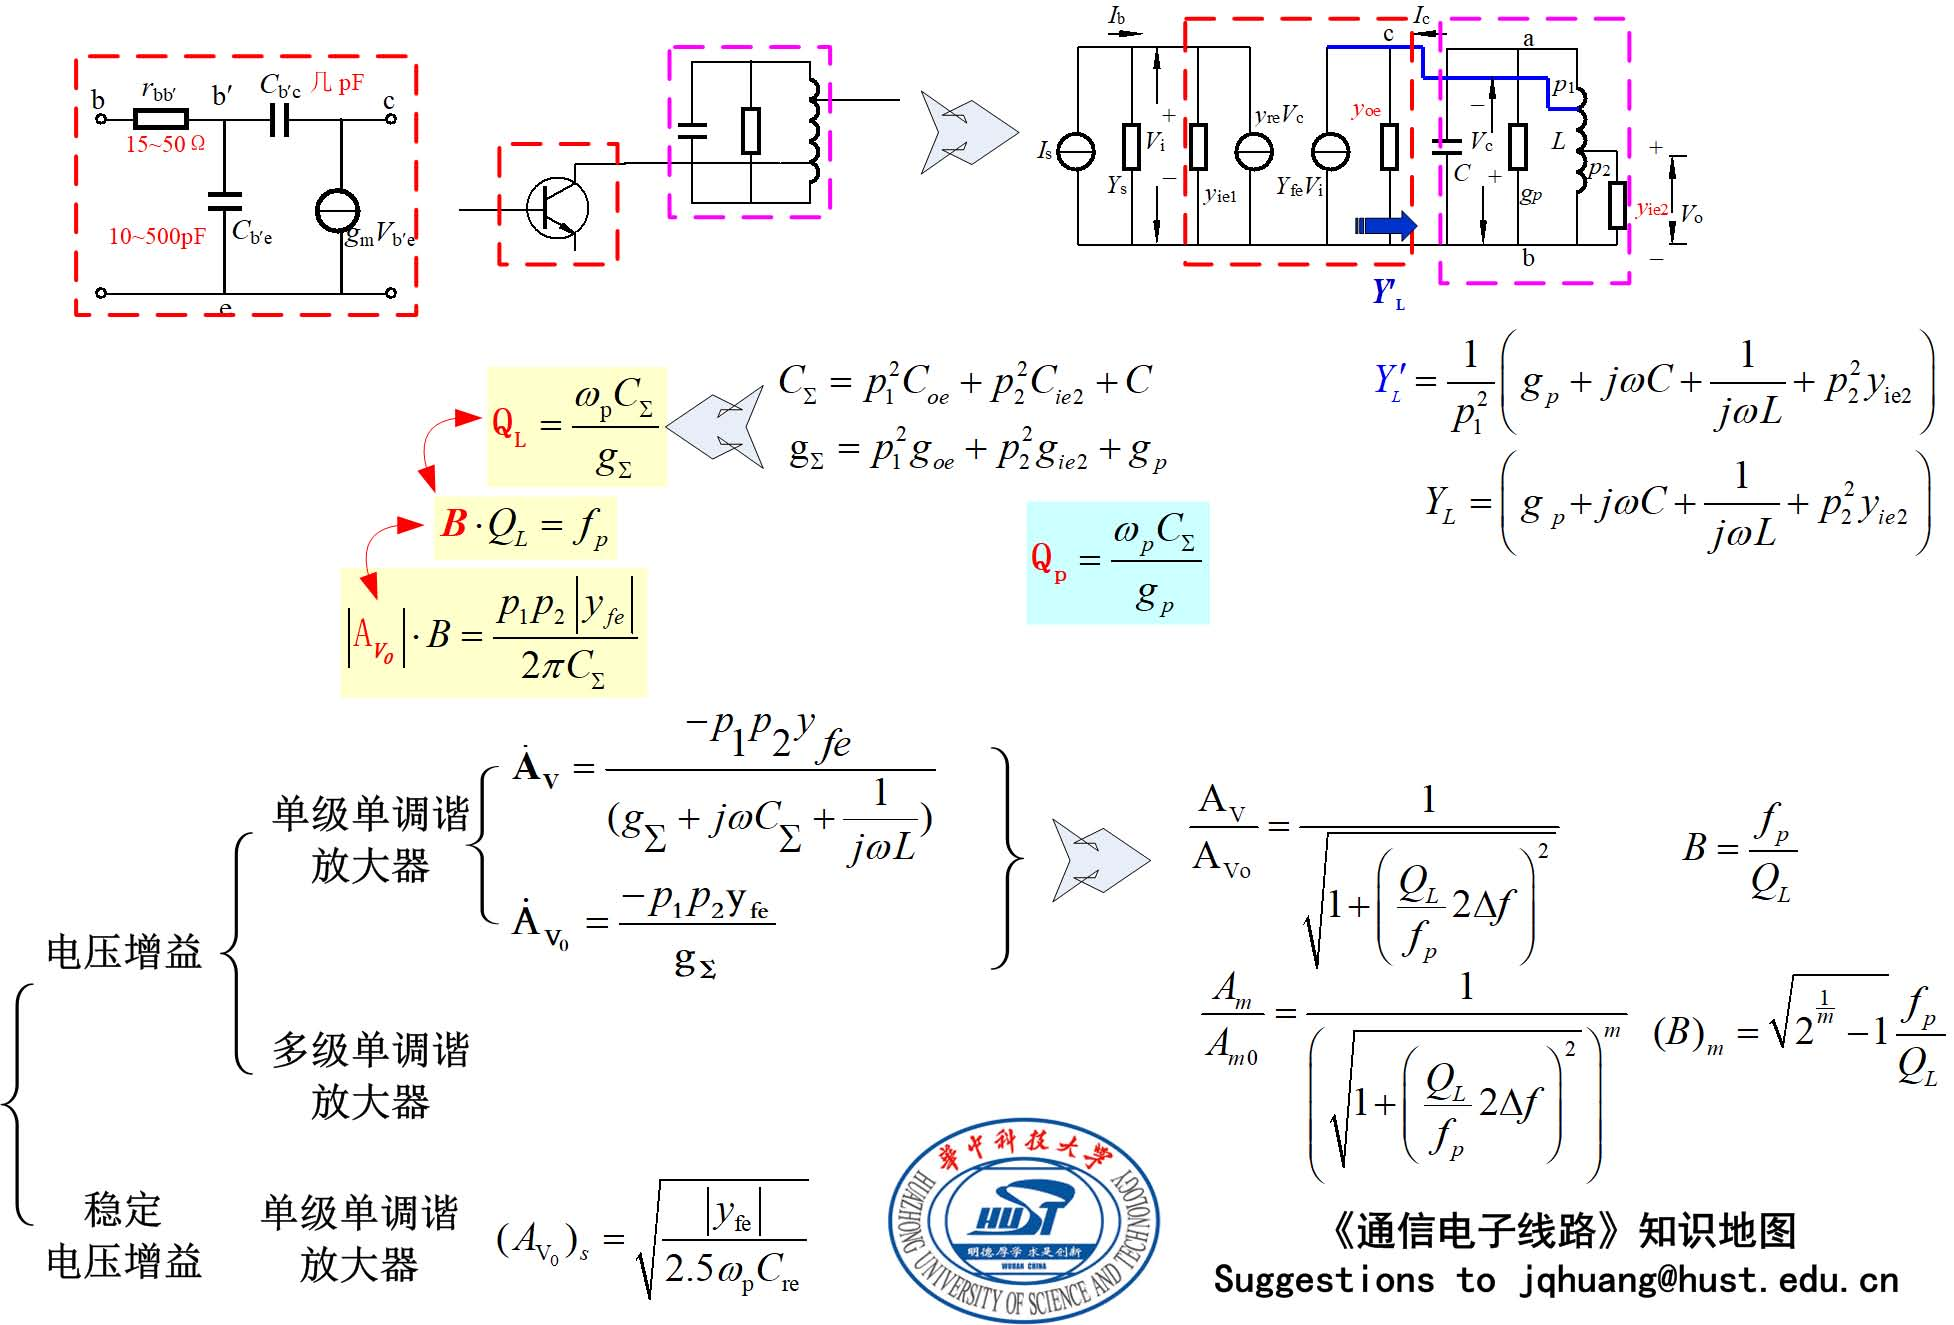
\includegraphics[width=1\textwidth]{small_amp_map.jpg}
\caption{知识地图}
\end{figure}

\chapter{混频}
\section{傅里叶分解}
电流$I$可以被分解为
\begin{itemize}
  \item 直流$I_0$
  \item 基波$I_{cm1}$
  \item $n$次谐波\footnote{直流成分可以被看做是0次谐波, 基波可以被看做是1次谐波}$I_{cmn}$
\end{itemize}
高频已调波信号和本机振荡信号经过混频后,信号中包含直流分量、基波分量、谐波、和频、差频分量\footnote{分别为$0,\,\omega_0,\,n\cdot\omega_0,\,\omega_0+\Omega,\,\omega_0-\Omega$},通过带通滤波器取出差频分量,完成混频。
\section{非线性电路}
时变参量电路的参数时按照一定规律随时间变化的. 
\subsection{幂级数分析法}
\subsection{折线分析法}
\section{混频过程}
一般来说中频$f_i$是一定的, 而本振频率$f_0$随着输入信号频率$f_s$而变化. 
\label{sec:mixing}
\begin{figure}[H]
\centering
\resizebox{\textwidth}{!}{

\begin{tikzpicture}
\coordinate (f_s) at (9,0);
\coordinate(f_p) at ($(f_s)+(1,0)$);
\coordinate(f_m) at ($(f_s)+(-1,0)$);
\coordinate (f_0) at (13,0);

\coordinate (f_i) at (4,0);
\coordinate(f_ip) at ($(f_i)+(1,0)$);
\coordinate(f_im) at ($(f_i)+(-1,0)$);

\draw [->] (0,0) node[below,left]{$O$}--(14,0) node[right]{$f$};
\draw [->] (0,0)--(0,2) node[right]{\small amplitude};
\draw [color=red] (f_s) node[below, text=black]{$f_s$}--+(0,1) node [draw=black, circle, fill=white,inner sep=1pt]{};
\draw [color=red] (f_p) node[below, text=black]{$f_s+F$}--+(0,.7) node [draw=black, circle, fill=white,inner sep=1pt]{};
\draw [color=red] (f_m) node[below, text=black]{$f_s-F$}--+(0,.7) node [draw=black, circle, fill=white,inner sep=1pt]{};

\draw [color=red] (f_0) node[below, text=black]{$f_0$}--+(0,1.8) node [draw=black, circle, fill=white,inner sep=1pt]{};

\draw [color=blue] (f_i) node[below, text=black]{$f_i$}--+(0,1) node [draw=black, circle, fill=white,inner sep=1pt]{};
\draw [color=blue] (f_ip) node[below, text=black]{$f_i+F$}--+(0,.7) node [draw=black, circle, fill=white,inner sep=1pt]{};
\draw [color=blue] (f_im) node[below, text=black]{$f_i-F$}--+(0,.7) node [draw=black, circle, fill=white,inner sep=1pt]{};

\draw ($(f_s)+(0,-0.5)$)--++(0,-.5);
\draw ($(f_0)+(0,-0.5)$)--++(0,-.5);
\draw [<->]  ($(f_s)+(0,-0.75)$)--node[below]{$f_i$}($(f_0)+(0,-0.75)$);

\draw ($(0,0)+(0,-0.5)$)--++(0,-.5);
\draw ($(f_i)+(0,-0.5)$)--++(0,-.5);
\draw [<->]  ($(0,0)+(0,-0.75)$)--node[below]{$f_i$}($(f_i)+(0,-0.75)$);
\end{tikzpicture}
}
\caption{频谱搬移}
\end{figure}
$f_i=f_0-f_s$ ($f_0>f_s$) $f_i$为中频频率, $f_0$为本地震荡频率, $f_s$为接收到的已调制信号的频率. (蓝色表示混频后, 红色表示混频前)\\
本振频率比外来信号频率高就是超外差, 与之对应的是超内差. 
外差就是频率变换 (混频) (和差化积公式). 
$$\cos(\alpha)\cdot \cos(\beta)=\frac{1}{2}\cdot [\cos(\alpha+\beta)+\cos(\alpha-\beta)]$$


\section{变频器}
混频器是一个三端器件,两个输入信号,一个输出信号
\subsection{晶体管混频器}
\subsection{二极管混频器}
\section{干扰}
\subsection{组合频率干扰}
combined frequency interference. 又被称作哨声干扰.
\begin{align*}
  f_s&\approx \frac{p\pm 1}{q-p}\cdot f_i
\end{align*}
$p,q$为任意正整数, 它们分别代表本振频率和信号频率的谐波次数.  
当中频信号一定时, 信号频率接近上式就可能会产生干扰哨声. 
\subsection{组合副波道干扰}
combined subchannel interference\\
副波道干扰为加性干扰, 即使没有输入信号仍然可以听见干扰噪声.
\subsubsection{副波道干扰}
常见的副波道干扰有中频干扰和镜像频率干扰.\\ 
\textbf{中频干扰}
\begin{align*}
  f_n\approx f_i
\end{align*} 
\textbf{镜像频率干扰}
\begin{align*}
  f_n&=f_0+f_i\\
  f_n-f_0&=f_i
\end{align*}
\subsection{交叉调制干扰 (交调)}
cross-modulation\\
乘性干扰, 就好像是干扰电台的调制信号转移到了有用信号的载波上. 
\subsection{互相调制干扰 (互调)}
两个或者更多个干扰信号同时加到接收机的输入端, 使得干扰信号彼此混频, 就可能产生频率接近有用信号频率的互调干扰(inter-modulation)分量. 
\subsection{阻塞干扰}
强干扰作用下晶体管工作于非线性区, 甚至完全破坏晶体管的工作状态
\subsection{外部干扰}
工业干扰\\
天线干扰
\subsection{干扰种类小结}
$f_s$为输入信号频率(signal), $f_i$为中频(intermediate), $f_n$为噪声频率(noise), $f_0$为谐振频率. \\
$n_s,n_0,n_n$为正整数, 其频率的整数倍. 
\begin{figure}[H]
\centering
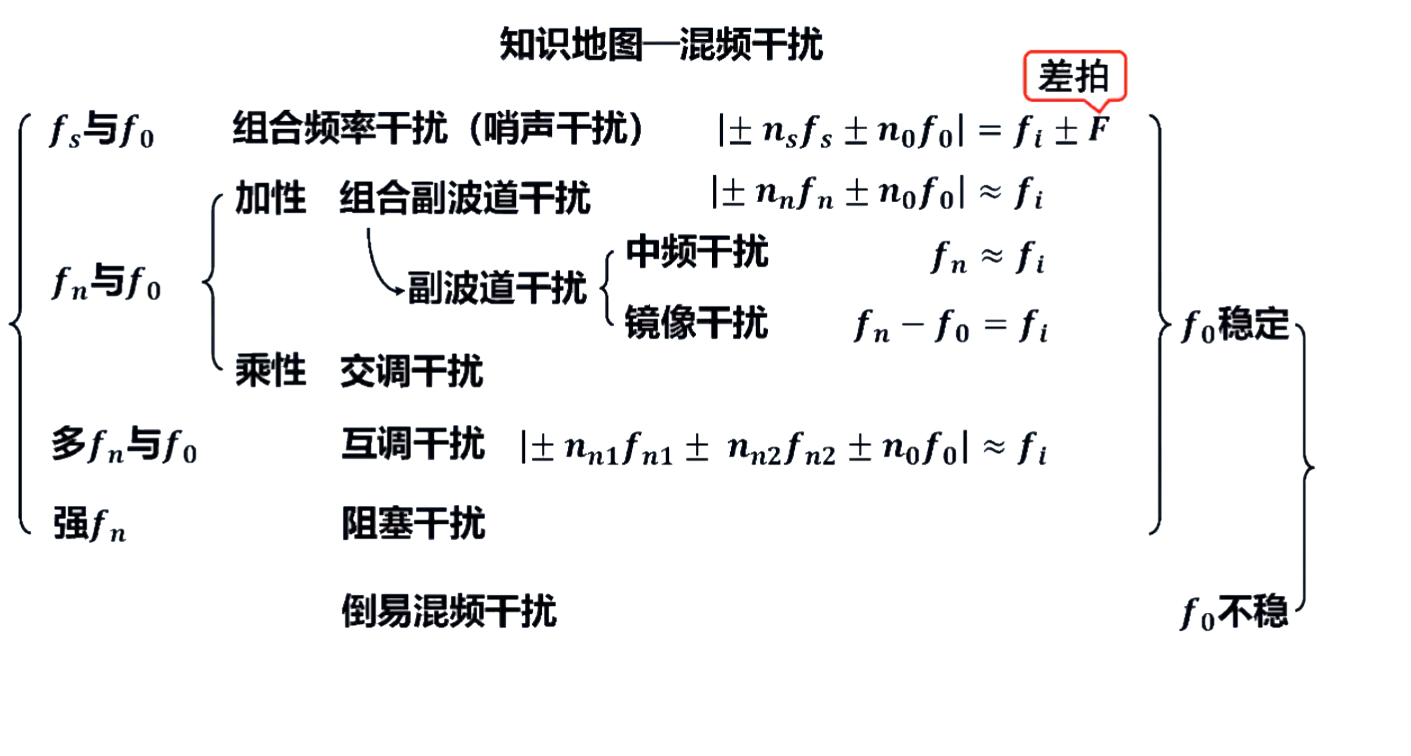
\includegraphics[width=\textwidth]{mix_noise_map.png}
\caption{混频干扰}
\end{figure}
\section{克服干扰的措施}
\begin{itemize}
  \item 提高前端电路的选择性
  \item 合理选择中频
  \item 合理选用电子器件与工作点 (BJT工作于三次非线性最小的区域)
\end{itemize}

\chapter{高频谐振功放}
用作发射机的最后一级功放
\section{特点}
\begin{itemize}
  \item 基极反偏
  \item 半导通角小于90度
  \item 产生尖顶余弦序列
  \item 由非线性的晶体管+线性的选频网络组合而成
\end{itemize}
工作在\textbf{非线性区}的BJT与\textbf{选频网络}组成
\subsection{与小信号放大器的比较}
\begin{figure}[H]
\centering
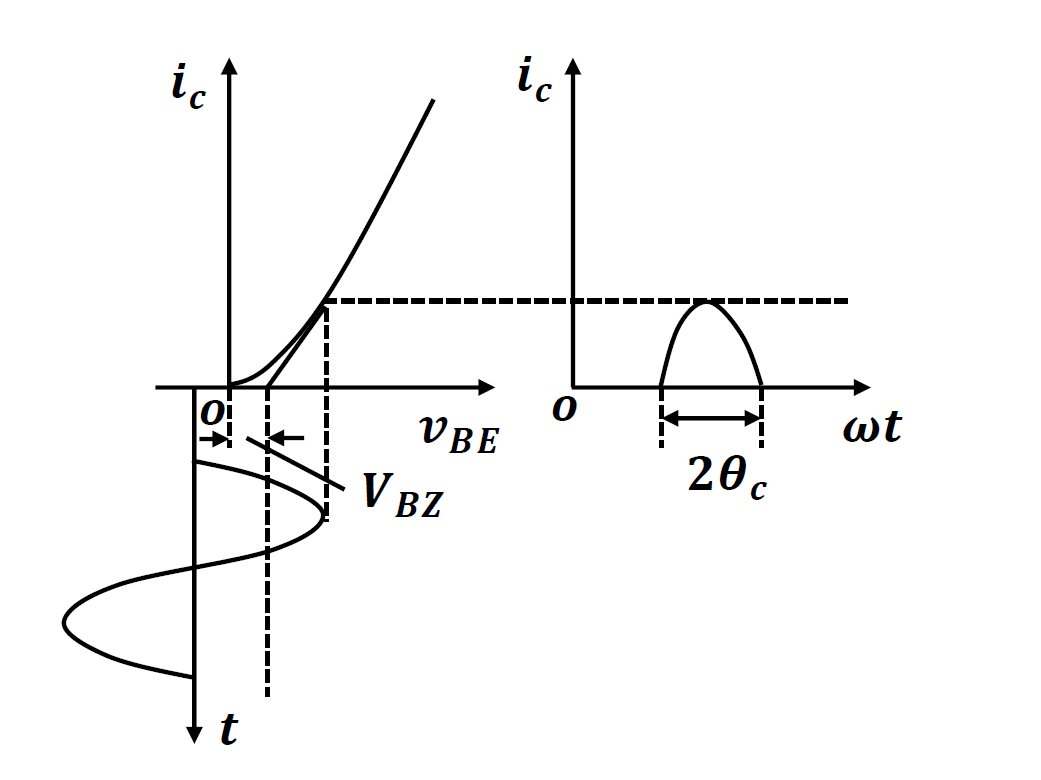
\includegraphics[width=0.5\textwidth]{power_amp_graph_1.png}
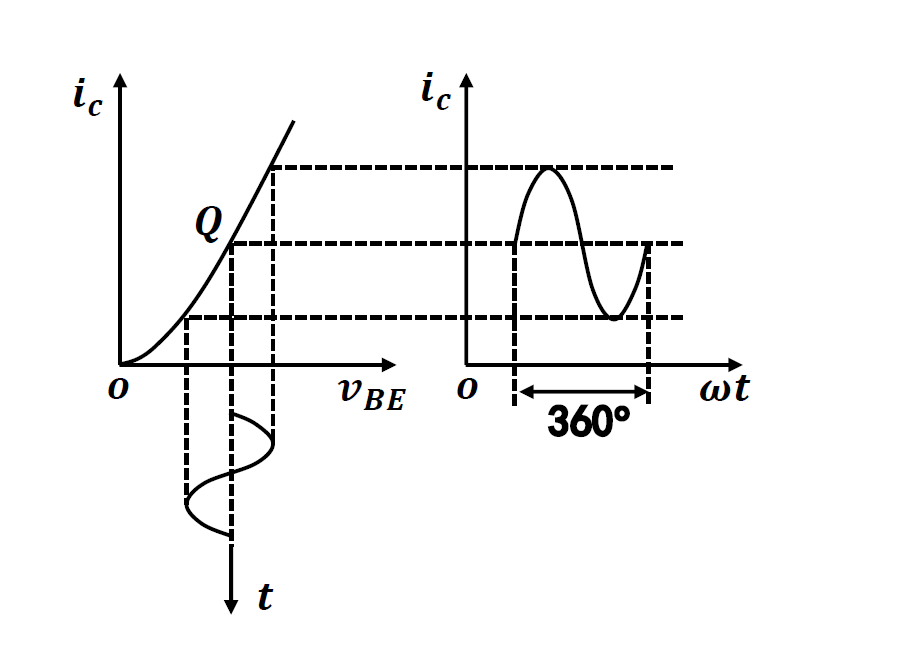
\includegraphics[width=0.5\textwidth]{power_amp_graph_2.png}
\caption{高频谐振功放(上)与高频谐振小放(下)}
\end{figure}
\paragraph{相同点}
\begin{itemize}
  \item 信号均为高频
  \item 负载均为谐振回路
\end{itemize}
\paragraph{不同点}
\begin{itemize}
  \item 激励信号的幅度大小不同
  \item 放大器的工作点不同
  \item 晶体管的动态范围不同
\end{itemize}
\begin{quote}
  \centering
  \textbf{反偏+丙类}($\theta_c<90^\circ$)
\end{quote}
\section{效率与功率}
高频谐振功放需要高功率和高效率
\subsection{输出功率}
\begin{align*}
  P_{\text{out}}&=P_{\text{直流}}-P_{\text{collector耗散}}\\
  &=P_{DC}-P_c\\
  &=\frac{1}{2}\cdot V_{cm}\cdot I_{cm1}
\end{align*}
具体计算公式看下面傅里叶分解. 
\begin{align*}
  P_{out}&=\frac{1}{2}\cdot V_{cm}\cdot I_{cm1}\\
  &=\frac{1}{2}\cdot \frac{V_{cm}^2}{R_p}\\
  &=\frac{1}{2}\cdot I_{cm1}^2\cdot R_p
\end{align*}
要提高输出功率就要降低集电极耗散功率. (还可提高集电极效率)
$$P_c=\frac{1}{T}\int_0^T i_C\cdot v_{CE} \;dt$$
\paragraph{降低$P_C$方法}
\begin{itemize}
  \item LC回路谐振在基频上 (使得$i_c$最大值正对$v_{CE}$最小值)
  \item 减小半导通角$\theta_c$
\end{itemize}
\subsection{集电极效率}
\begin{align*}
  \eta_c=\eta_{\text{collector}}=\frac{P_{\text{out}}}{P_{\text{直流}}}&=\frac{P_{\text{out}}}{P_{\text{out}}+P_{\text{collector耗散}}}\\
  &=\frac{P_o}{P_o+P_c}\\
  P_\text{out}&=(\frac{\eta_c}{1-\eta_c}\cdot P_c)
\end{align*}
具体计算公式看下面傅里叶分解. 
\subsection{导通角}
\begin{align*}
  \cos(\theta_c)&=\frac{V_{\text{基级偏置电压}}+V_{\text{晶体管导通电压}}}{V_{\text{基级交流信号电压振幅}}}\\
  &=\frac{V_{BB}+V_{BZ}}{V_{bm}}
\end{align*}
\section{傅里叶分解集电极电流}
$$i_c=I_{c0}+I_{cm1}\cdot\cos(\omega t)+I_{cm2}\cdot\cos(2\omega t)\dots +I_{cmn}\cdot\cos(n\omega t)$$
$I_{c0}$为直流成分, $I_{cmn}$为$n$次谐波. 
\subsection{输出功率}
\begin{align*}
  P_0&=\frac{1}{2}\cdot V_{cm}\cdot I_{cm1}\\
  &=\frac{1}{2} \frac{V_{cm}^2}{R_p}\\
  &= \frac{1}{2}I_{cm1}^2\cdot R_p
\end{align*}

\subsection{集电极效率}
\begin{align*}
  \eta_c&=\frac{P_o}{P_=}\\
  &=\frac{\frac{1}{2}\cdot V_{cm}\cdot I_{cm1}}{V_{CC}\cdot I_{c0}}\\
  &=\frac{1}{2}\cdot \underset{\text{集电极电压利用系数$\xi$}}{\frac{V_{cm}}{V_{CC}}}
  \cdot \underset{\text{波形系数$g_1(\theta_c)$}}{\frac{I_{cm1}}{I_{c0}}}\\
  &=\frac{1}{2}\cdot \xi\cdot g_1(\theta_c)
\end{align*}
那么问题来了, 怎么求$I_{cm1}$和$I_{c0}$. 当然是傅里叶分解尖顶余弦脉冲$i_c$序列啦
$$i_c=I_{c0}+I_{cm1}\cdot\cos(\omega t)+I_{cm2}\cdot\cos(2\omega t)\dots +I_{cmn}\cdot\cos(n\omega t)$$
$I_{c0}$为直流成分, $I_{cmn}$为$n$次谐波. \\
使用\textbf{折线近似法} (从转移特性和输出特性入手) 来得到所需的尖顶余弦电流脉冲
\subsection{尖顶余弦脉冲}
由于集电极负载的\textbf{选频}作用,输出的是与输入信号频率相同的\textbf{余弦波}。

谐振功率放大器工作在丙类状态,所以集电极电流为周期性的余弦脉冲波形,但其负载为调谐回路谐振在基波频率,可选出集电极的基波电流,故在负载两端可得到电压仍为与信号同频的余弦波电压
\subsubsection{折线近似法}
\begin{figure}[H]
\centering
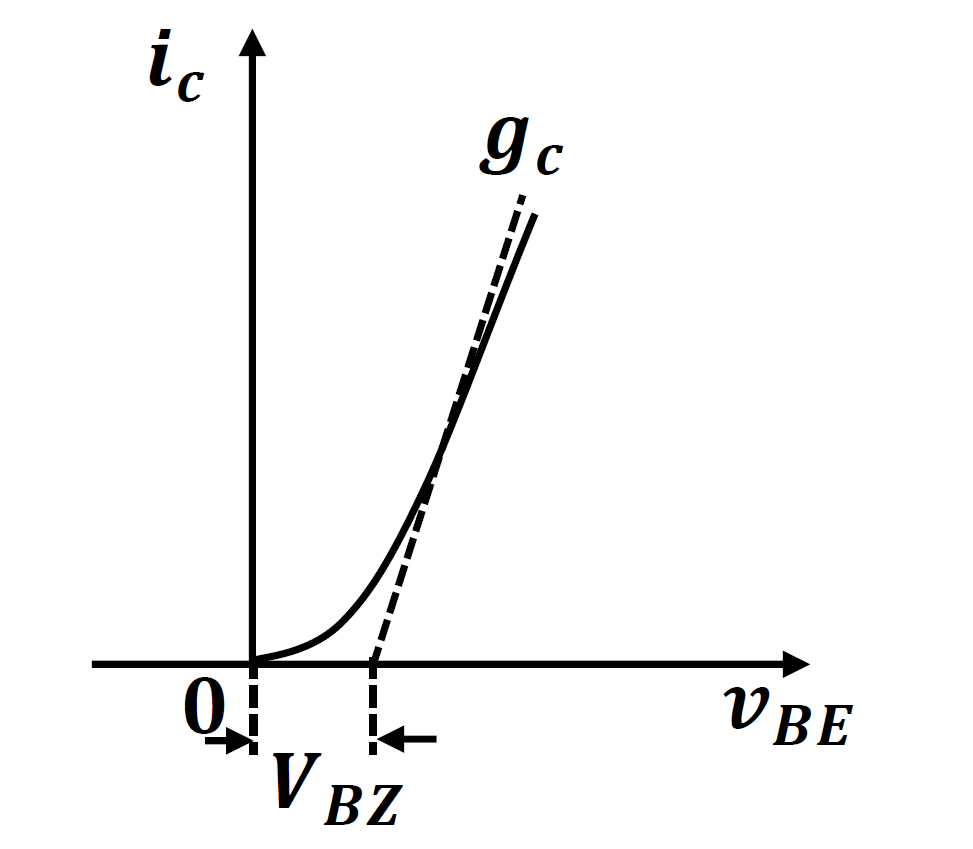
\includegraphics[width=0.4\textwidth]{power_amp_graph_4.png}
\caption{输出特性曲线}
\end{figure}
\begin{figure}[H]
\centering
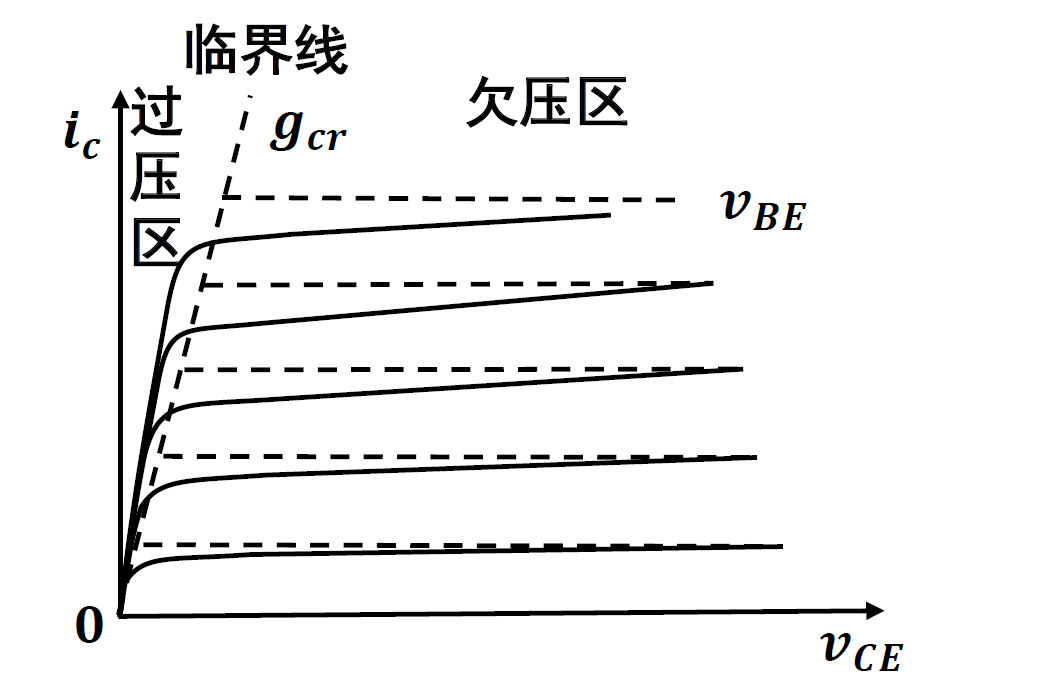
\includegraphics[width=0.4\textwidth]{power_amp_graph_5.png}
\caption{转移特性曲线}
\end{figure}
所谓折线近似法就是将输出特性曲线和转移特性曲线的临界线视为折线而非曲线. 
\begin{align*}
  i_c&=g_m\cdot(v_{BE}-V_{BZ}) &&\text{转移特性方程}\\
  i_c&=g_m\cdot v_{CE}&&\text{临界线方程}
\end{align*}\footnote{图中跨导以$g_c$标识, 但我更习惯用$g_m$}
过程略, 结果如下\footnote{完整的图像从解析式画出来应该是一个余弦波, 但是这里仅仅截取大于0的部分}

\begin{align*}
  \cos(\theta_c)&=\frac{V_{BB}+V_{BZ}}{V_{bm}}\\
  i_c&=i_{\text{cmax}}\cdot \frac{\cos(\omega t)-\cos(\theta_c)}{1-\cos(\theta_c)}&&\text{尖顶余弦脉冲的解析式}\\
  i_{\text{cmax}}&=g_m\cdot V_{bm}\cdot (1-\cos(\theta_c))&&\text{通过跨导和输入电压的最大值求出}\\
  i_\text{cmax}&=g_m\cdot (V_{CC}-V_{cm})\\
  g_m&=\text{输出特性曲线的斜率}=\text{转移特性的临界线的斜率}
\end{align*}

\begin{figure}[H]
\centering
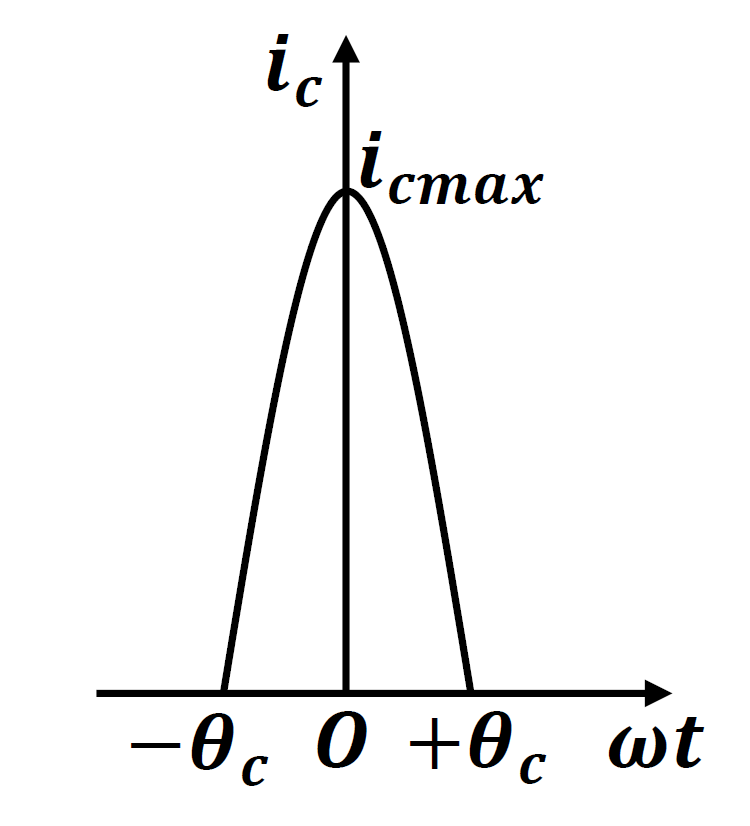
\includegraphics[width=0.4\textwidth]{power_amp_graph_3.png}
\caption{尖顶余弦脉冲 ($i_c<0$部分被截去)}
\end{figure}
对上式进行傅里叶展开, 可以求得系数. 分解系数是关于导通角$\theta_c$的函数. 
\begin{figure}[H]
\centering

\definecolor{qqwuqq}{rgb}{0,0.39215686274509803,0}
\definecolor{ffqqqq}{rgb}{1,0,0}
\definecolor{qqzzff}{rgb}{0,0.6,1}
\pgfplotsset{compat=1.15}
\begin{tikzpicture}
\begin{axis}[
%x=1cm,y=1cm,
axis lines=middle,
ymajorgrids=true,
xmajorgrids=true,
xmin=0,
xmax=3.1415926535897,
ymin=0,
ymax=2,
xtick={-1,-0.5,...,5},
ytick={-1.5,-1,...,3},
xlabel={$\theta_c$},
ylabel={$\alpha_n$ or $\frac{\alpha_1}{\alpha_0}$}
]
%\clip(-1.079802977970752,-1.6933439296602872) rectangle (5.048730801308572,3.133377118726336);
\draw[color=qqzzff,smooth,samples=100,domain=0.1:pi] plot(\x,{(sin(((\x))*180/pi)-(\x)*cos(((\x))*180/pi))/(3.141592653589793*(1-cos(((\x))*180/pi)))});
%\draw [line width=2pt] (3.141592653589793,-1.6933439296602872) -- (3.141592653589793,3.133377118726336);
\draw[color=ffqqqq,smooth,samples=100,domain=0:pi] plot(\x,{((\x)-sin(((\x))*180/pi)*cos(((\x))*180/pi))/(3.141592653589793*(1-cos(((\x))*180/pi)))});
\draw[color=qqwuqq,smooth,samples=100,domain=0:pi] plot(\x,{((\x)-sin(((\x))*180/pi)*cos(((\x))*180/pi))/(3.141592653589793*(1-cos(((\x))*180/pi)))/((sin(((\x))*180/pi)-(\x)*cos(((\x))*180/pi))/(3.141592653589793*(1-cos(((\x))*180/pi))))}) ;
% \begin{scriptsize}
 \draw[color=red] (1.5,0.5) node[above] {$\alpha_1$};
 \draw[color=blue] (2,0) node[above] {$\alpha_0$};
 \draw[color=qqwuqq] (0.5,1.5) node {$\frac{\alpha_1}{\alpha_0}$};
% \end{scriptsize}
\end{axis}
\end{tikzpicture}

\caption{尖顶脉冲的分解系数 (懒得画$\alpha_3$以上的了)}
\end{figure}
还记得波形系数么? 
$$g_1(\theta_c)=\frac{I_{cm1}}{I_{c0}}=\frac{\alpha_1(\theta_c)}{\alpha_0(\theta_c)}$$
为了兼顾功率和效率, 最佳$\theta_c=70^\circ$左右. 
\section{高频功放理论小结}
\begin{figure}[H]
\centering
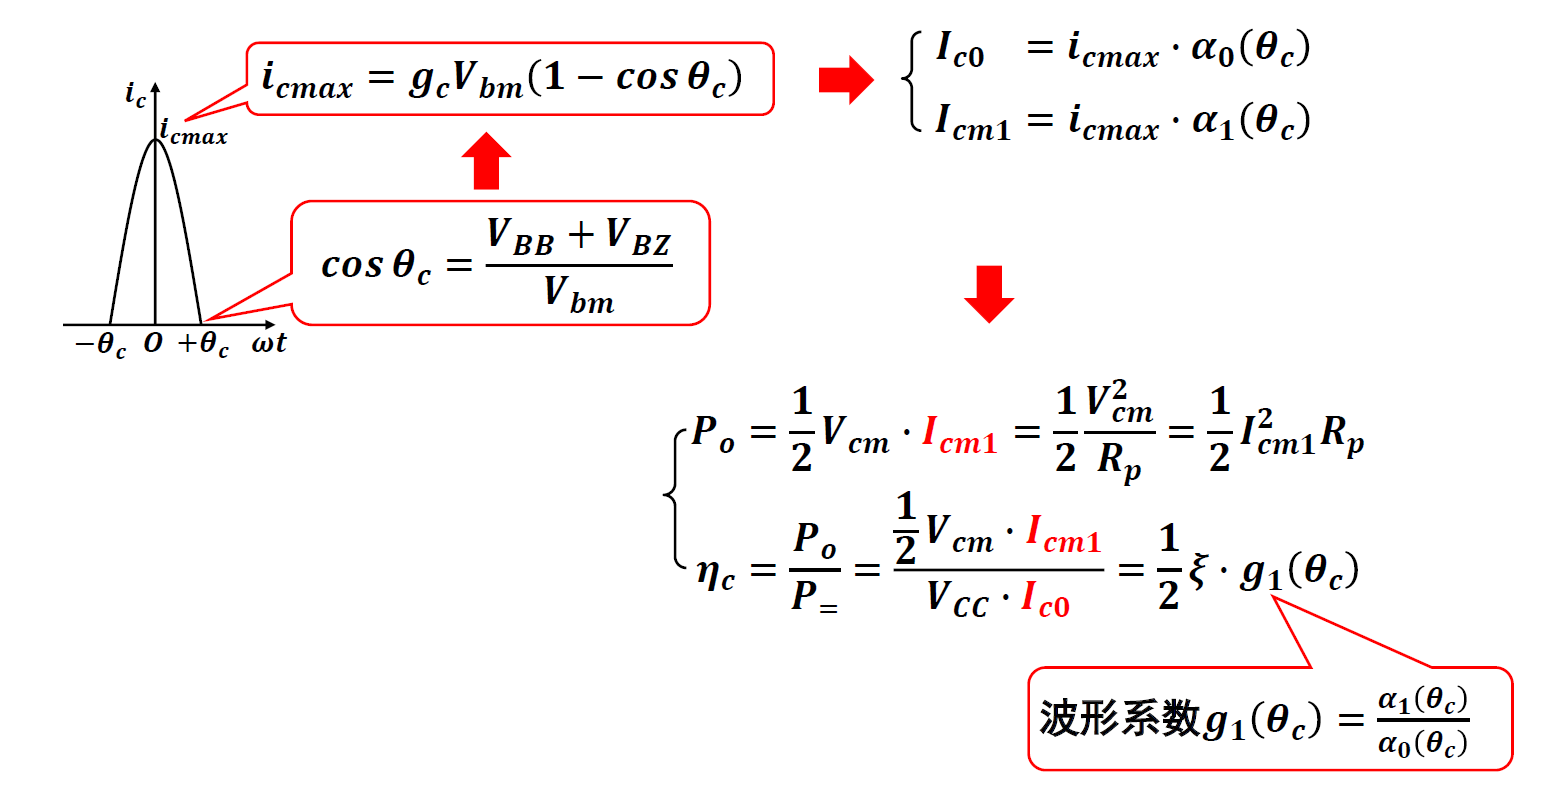
\includegraphics[width=1\textwidth]{power_amp_map_1.png}
\caption{小结}
\end{figure}
\begin{figure}[H]
\centering
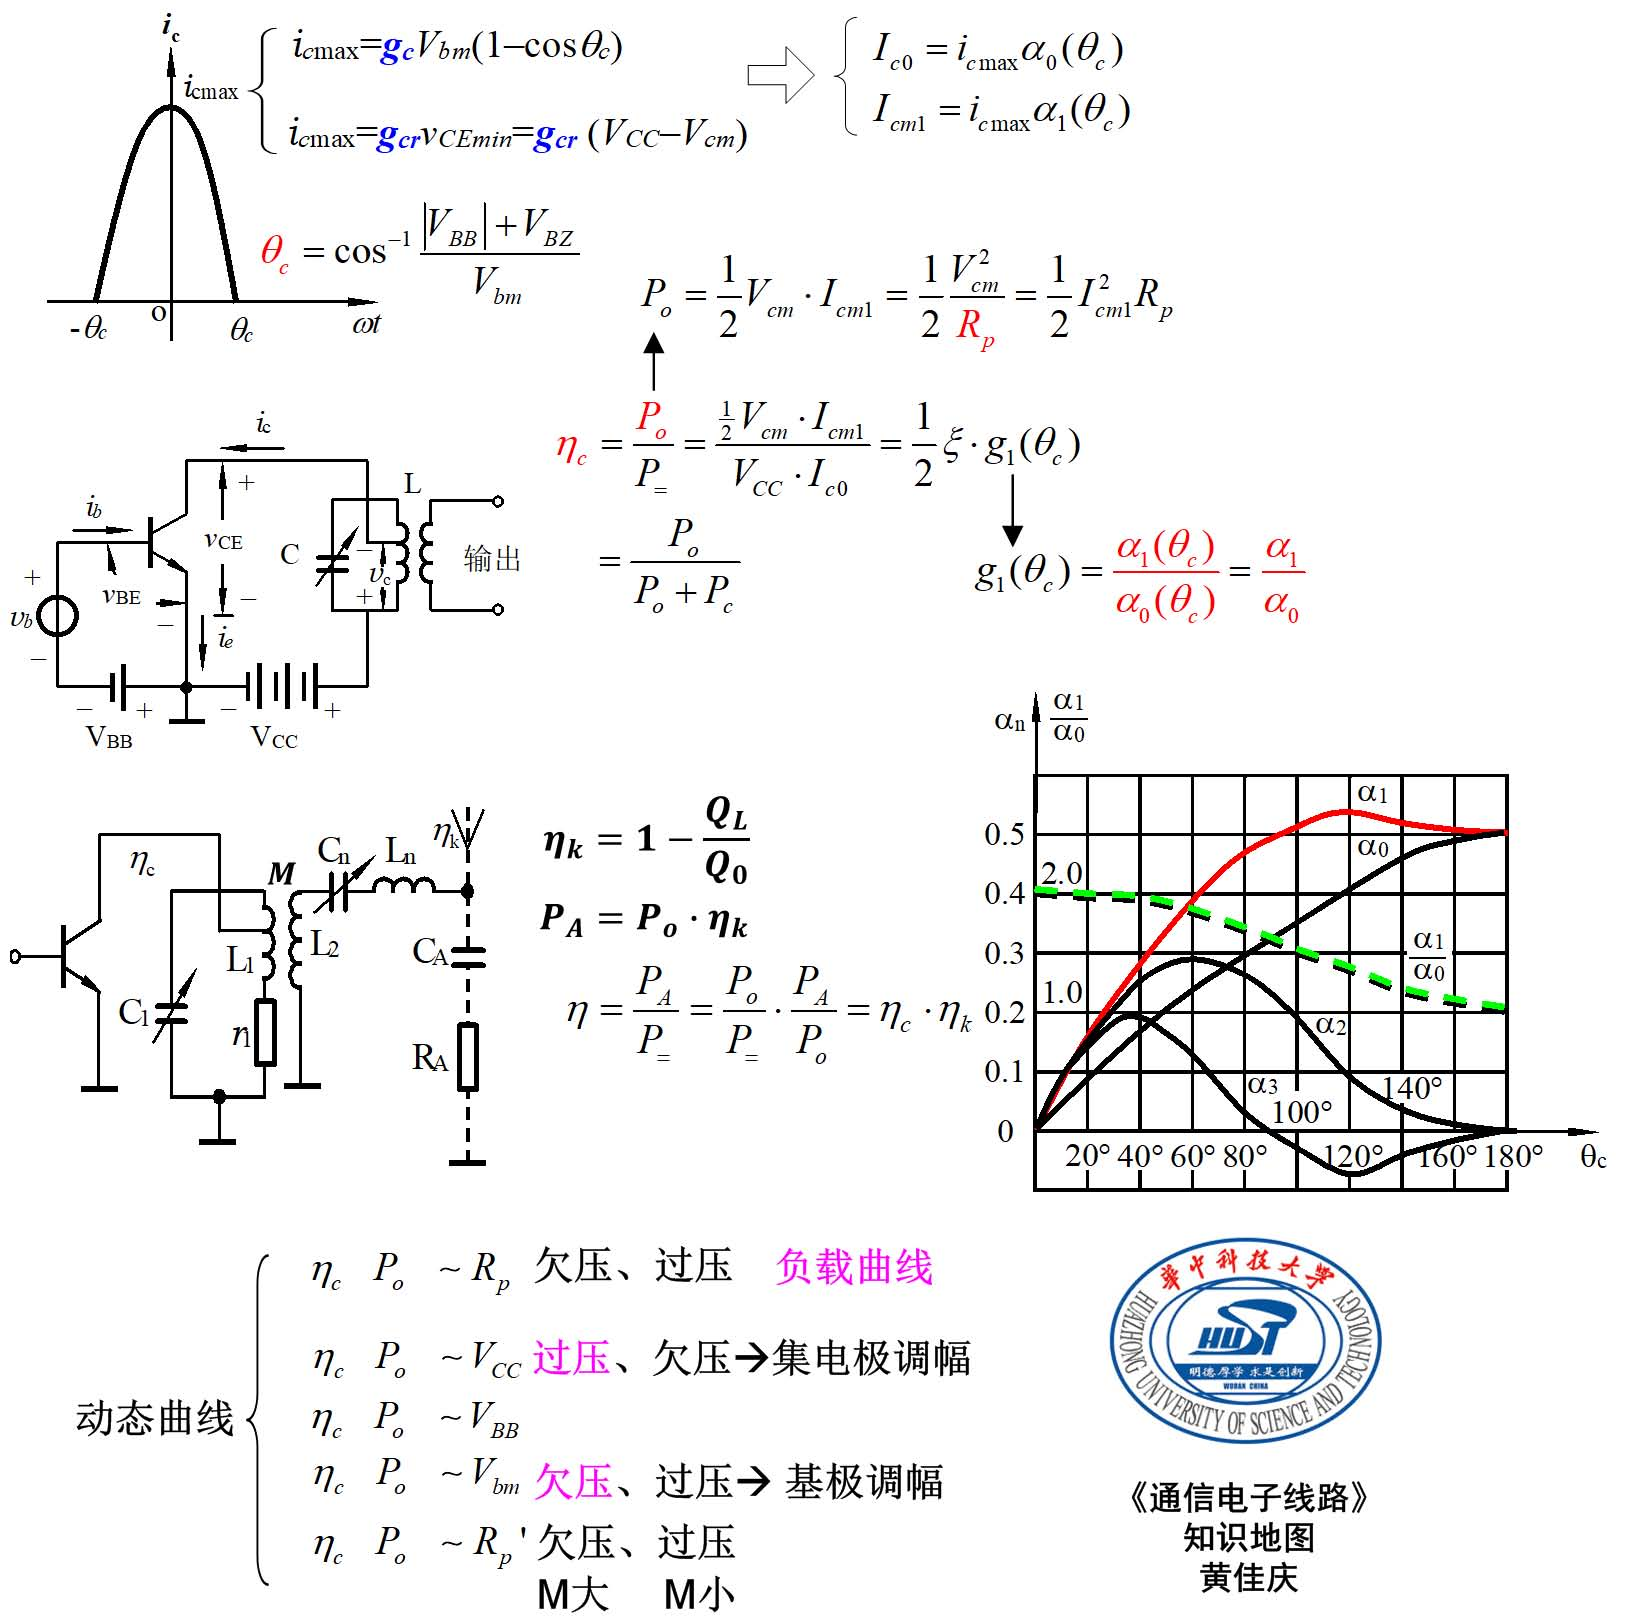
\includegraphics[width=1\textwidth]{power_amp_map_2.jpg}
\caption{知识地图}
\end{figure}

\section{负载特性和动态特性}
$R_p$为集电极谐振回路的谐振电阻. $R_p=\frac{L}{RC}$
\begin{itemize}
  \item 当高频谐振功率放大器的集电极电流都在临界线的右方时,称为欠压工作状
  态
  \item 当集电极电流的最大值正好落在临界线上时,称为临界工作状态
  \item 当集电极电流的最大值穿过了临界线到达左方饱和区时,称为过压工作状态。
\end{itemize}
\subsection{并联谐振回路电阻$R_p$}
\begin{figure}[H]
\centering
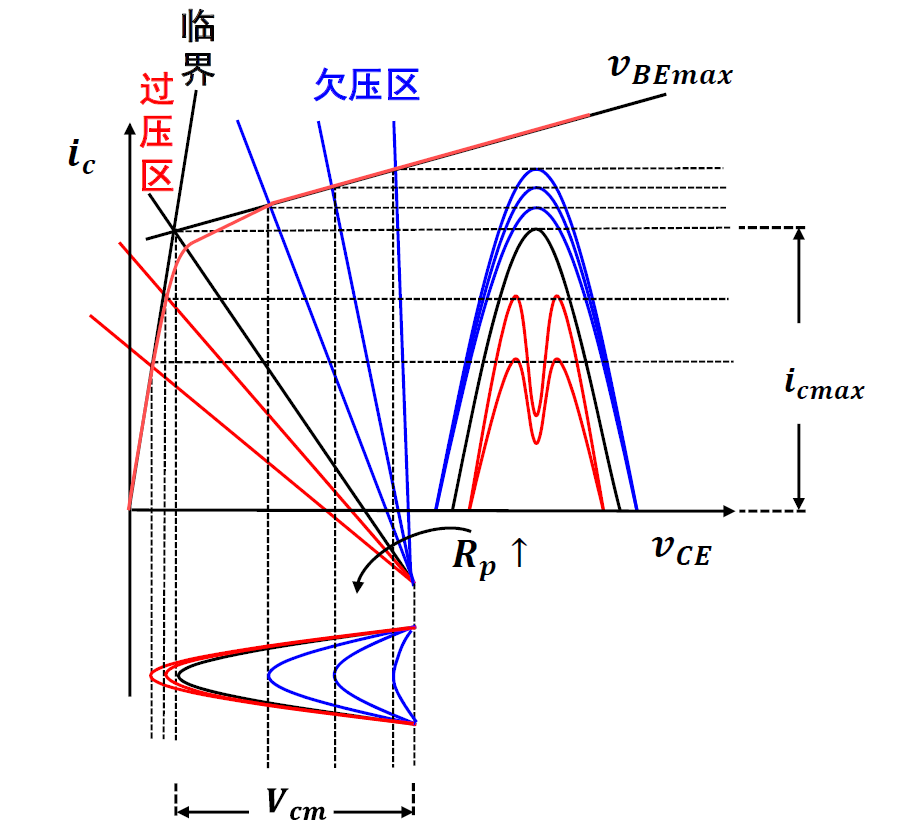
\includegraphics[width=0.5\textwidth]{power_amp_graph_6.png}
\caption{$R_p$的动态特性曲线}
\end{figure}
\begin{figure}[H]
\centering
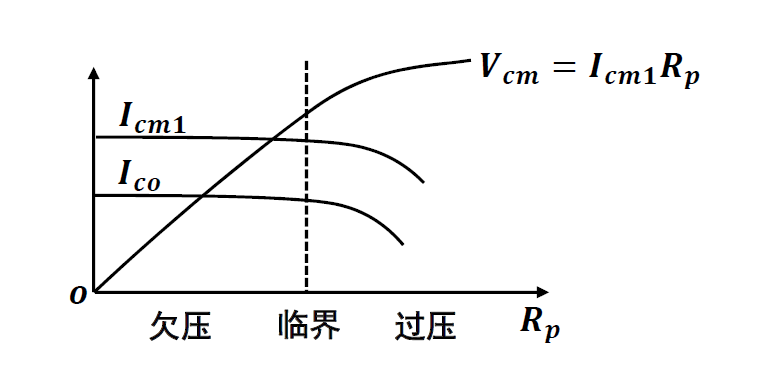
\includegraphics[width=0.4\textwidth]{power_amp_graph_7.png}
\caption{$R_p$对集电极电压以及电流的影响 (负载特性)}
\end{figure}
\begin{figure}[H]
\centering
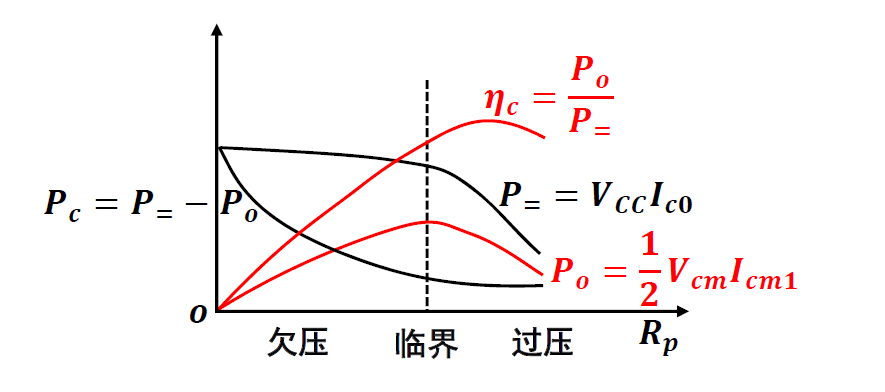
\includegraphics[width=0.5\textwidth]{power_amp_graph_8.png}
\caption{$R_p$对功率的影响 (负载特性)}
\end{figure}
从欠压到过压. 
\begin{itemize}
  \item 欠压
  \item 临界 $P_o$可达最高, 为最佳工作状态, 常用作发射机末级
  \item 过压 $\eta_c$可达最高, 常用作中间放大级 (且输出电流平稳)
\end{itemize}
\subsection{直流电源电压 $V_{CC}$}
\begin{figure}[H]
  \centering
  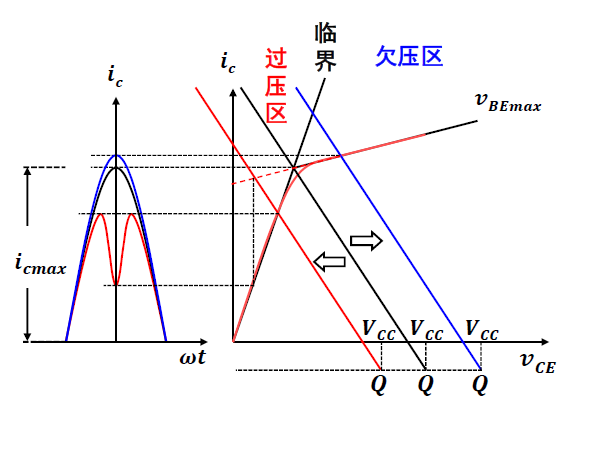
\includegraphics[width=0.5\textwidth]{power_amp_graph_vcc_1.png}
  \caption{$V_{CC}$的动态特性曲线}
  \end{figure}
  \begin{figure}[H]
  \centering
  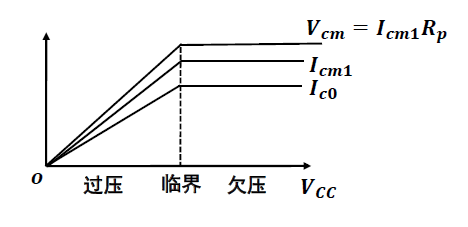
\includegraphics[width=0.4\textwidth]{power_amp_graph_vcc_2.png}
  \caption{$V_{CC}$对集电极电压以及电流的影响}
  \end{figure}
  \begin{figure}[H]
  \centering
  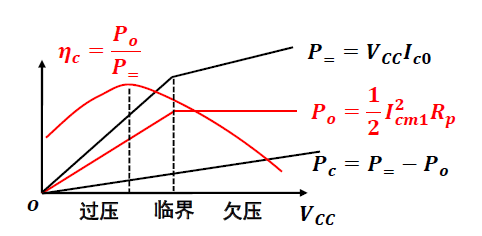
\includegraphics[width=0.4\textwidth]{power_amp_graph_vcc_3.png}
  \caption{$V_{CC}$对功率的影响}
  \end{figure}
从过压到欠压

\subsection{输入信号振幅$V_{bm}$}
\begin{figure}[H]
\centering
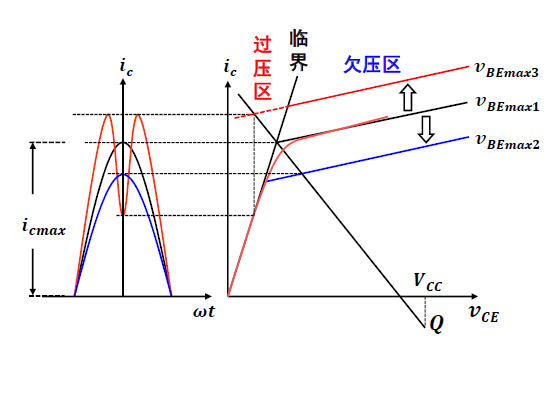
\includegraphics[width=0.5\textwidth]{power_amp_graph_vbm_1.png}
\caption{$V_{bm}$的动态负载特性曲线}
\end{figure}
\begin{figure}[H]
\centering
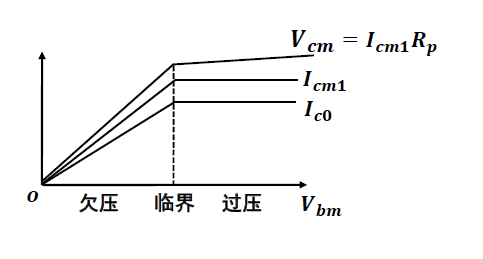
\includegraphics[width=0.4\textwidth]{power_amp_graph_vbm_2.png}
\caption{$V_{bm}$的负载特性曲线 (电压电流)}
\end{figure}
\begin{figure}[H]
\centering
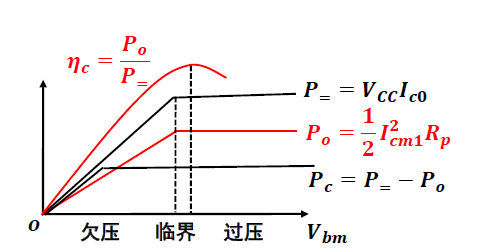
\includegraphics[width=0.4\textwidth]{power_amp_graph_vbm_3.png}
\caption{$V_{bm}$的负载特性曲线 (功率效率)}
\end{figure}
从欠压到过压. ($V_{bm}\uparrow,|\mathbb{V}_{BB}|\downarrow$)
和$V_{CC}$的特性曲线很像, $V_{CC}$是从over到under. $V_{bm}$是从under到over. 
\section{直流馈电电路}
\subsection{集电极馈电电路}
指$V_{CC}$, 谐振回路, BJT三者连接的一种直流馈电电路

\subsubsection{串联馈电}
指$V_{CC}$, 谐振回路, BJT三者首尾相连的一种直流馈电电路
\begin{figure}[H]
\centering
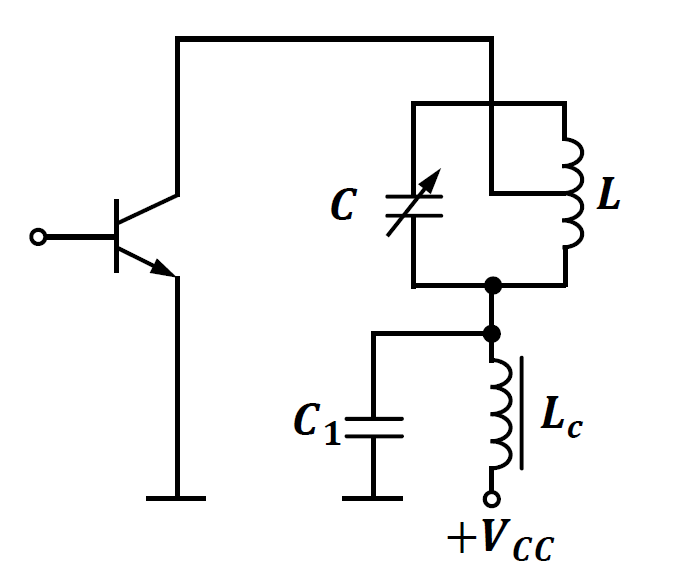
\includegraphics[width=0.4\textwidth]{power_res_fb_c_s.png}
\caption{集电极串联馈电}
\end{figure}

\paragraph{优点} $L_c$处于高频零电位, 对地分布电容不影响频率稳定性
\paragraph{缺点} 回路电容$C$上有高压
\subsubsection{并联馈电}
指$V_{CC}$, 谐振回路, BJT三者并联连接的一种直流馈电电路
\begin{figure}[H]
  \centering
  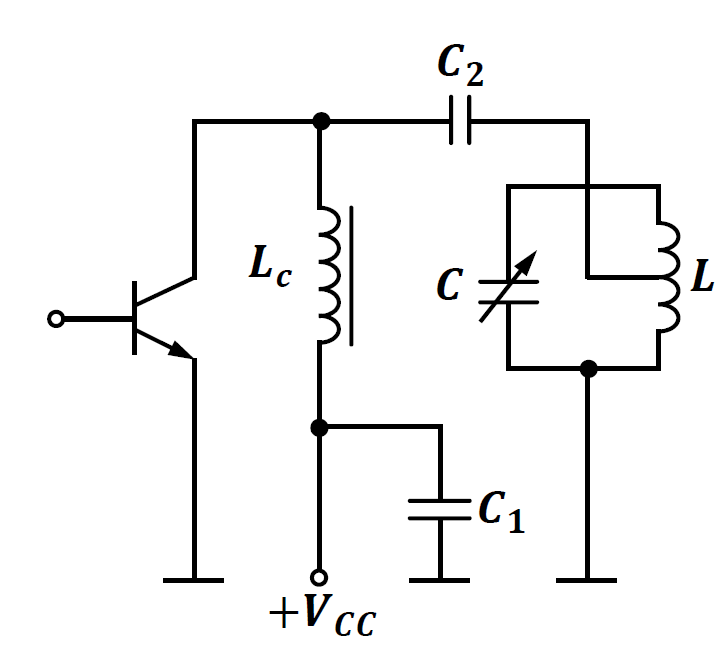
\includegraphics[width=0.4\textwidth]{power_res_fb_c_p.png}
  \caption{集电极并联馈电}
  \end{figure}
  \paragraph{优点} 回路电容$C$上无高压, 安全可靠
  \paragraph{缺点} $L_c$处于高频高电位, 对地分布电容对频率稳定性较大

\subsection{基极馈电电路}
指$V_{BB}$, 信号源, BJT三者连接的一种直流馈电电路
\subsubsection{串联馈电}
\begin{figure}[H]
  \centering
  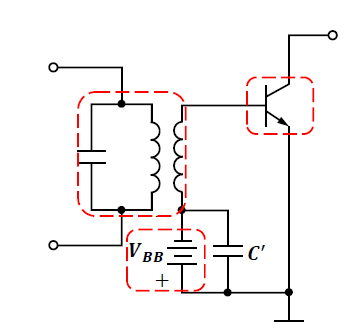
\includegraphics[width=0.4\textwidth]{power_res_fb_b_s.png}
  \caption{基级串联馈电}
  \end{figure}
\subsubsection{并联馈电}
\begin{figure}[H]
  \centering
  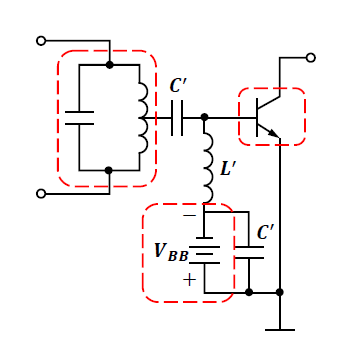
\includegraphics[width=0.4\textwidth]{power_res_fb_b_p.png}
  \caption{基级并联馈电}
  \end{figure}

\section{级间耦合电路}
对于中间级而言,最主要的是应该保证它的电压输出稳定,以供给下级功放稳定的激励电压,而效率则降为次要问题。
\begin{itemize}
  \item 使中间级放大器工作于过压状态,使它近似为一个恒压源。
  \item 降低级间耦合回路的效率。回路效率降低后,其本身的损耗加大。这样下级输入阻抗的变化相对于回路本身的损耗而言就不显得重要了。
\end{itemize}
\subsection{输出匹配网络}
\subsubsection{中介回路效率$\eta_k$}
\begin{align*}
  \eta_k&=\frac{\text{输出至负载的有效功率}}{\text{输入到回路的总交流功率}}\\
  P_\text{antenna}&=P_o\cdot \eta_k
\end{align*}

\chapter{Oscillator}
\section{条件}
\subsection{起振条件}
\begin{align*}
  \mathbb{A}\cdot\mathbb{F}>1\\
  \begin{cases}
    A\cdot F>1\\
    \phi_A+\phi_F=2n\pi
  \end{cases}
\end{align*}
\subsection{平衡条件}
\begin{align*}
  \mathbb{A}\cdot\mathbb{F}=1\\
  \begin{cases}
    A\cdot F=1\\
    \phi_A+\phi_F=2n\pi
  \end{cases}
\end{align*}
\subsection{稳定条件}
\paragraph{软激励起振} 初始激励$A_0$, 平均增益$A$
\begin{figure}[H]
\centering
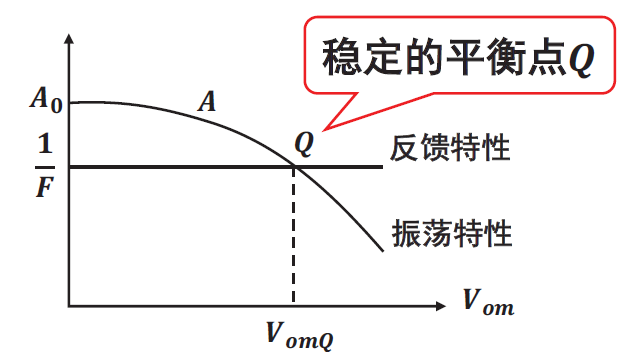
\includegraphics[width=0.4\textwidth]{osc_condition_1.png}
\caption{软激励起振}
\end{figure}
\paragraph{硬激励起振} $A_0$过小, 不能自行起振, 需要增加初始激励
\begin{figure}[H]
\centering
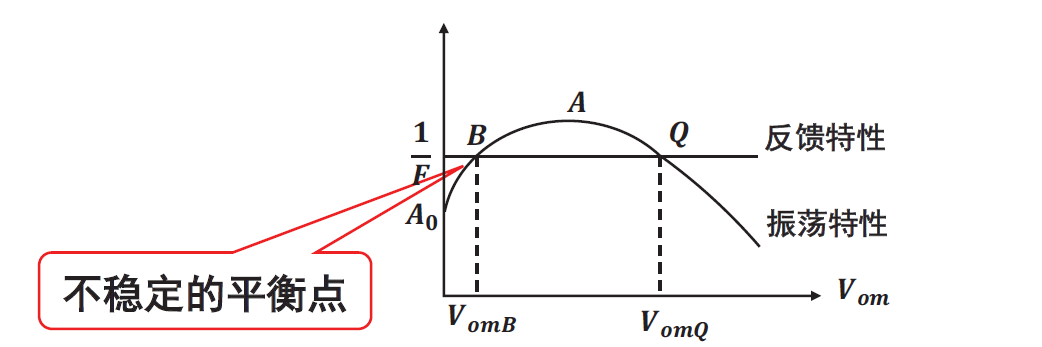
\includegraphics[width=0.6\textwidth]{osc_condition_2.png}
\caption{硬激励起振}
\end{figure}

\begin{align*}
  \frac{\partial A }{\partial V_{om}}|_{V_{om}=V_{omQ}}&<0&&\text{在平衡点附近, 增益$A$随振幅的变化具有负斜率}\\
  \frac{\partial \phi }{\partial \omega}&<0 &&\text{在平衡点附近, 相频特性曲线随频率变化特性具有负的斜率}
\end{align*}
两个负斜率
\begin{itemize}
  \item 增益$A$与振幅$V_{om}$的输出曲线
  \item 相频特性曲线随频率的变化特性 See Section~\ref{sec:omega_phi_graph}
\end{itemize}
\section{互感耦合振荡器}
\paragraph{优点} 在调整反馈系数时, 基本不影响振荡频率. 
\paragraph{缺点} 工作频率不宜过高, 一般应用于中短波. 因为存在分布电容, 频率较高时, 难以做出稳定性高的变压器.
\paragraph{难点} 判断是否起振: 确定$\mathbb{V}_f$ (由$\mathbb{V}_f=\mathbb{V}_i$)
\subsection{Base}
调基 (部分接入)
\begin{figure}[H]
\centering
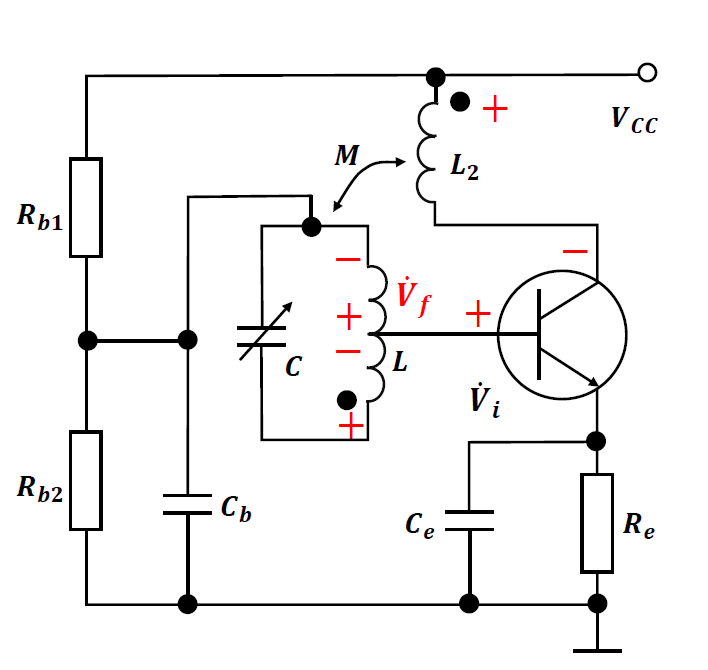
\includegraphics[width=0.33\textwidth]{osc_lc_base.png}
\caption{调基电路}
\end{figure}
部分接入原因
\begin{itemize}
  \item 基级于发射级之间的输入阻抗较低
  \item 减少对谐振回路Q值的影响
\end{itemize}

\subsection{Emitter}
调发 (部分接入)
\begin{figure}[H]
  \centering
  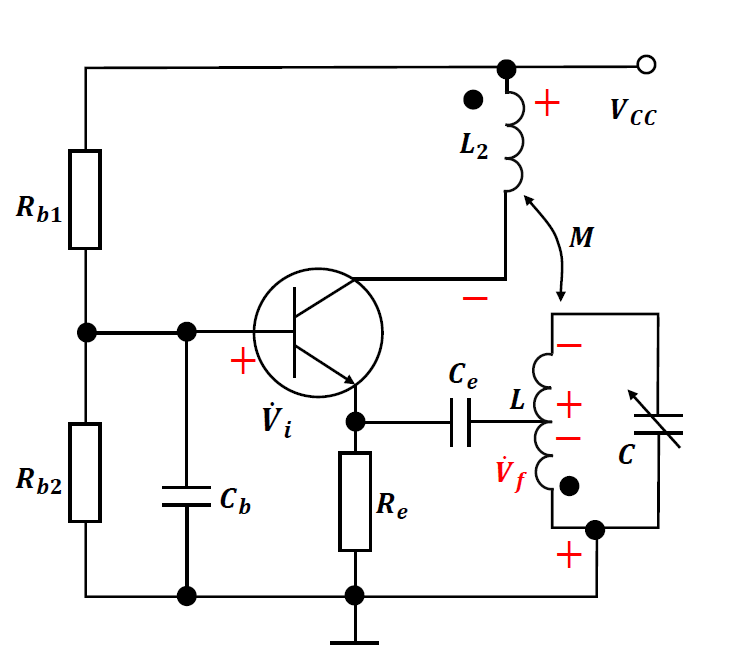
\includegraphics[width=0.33\textwidth]{osc_lc_emitter.png}
  \caption{调发电路}
  \end{figure}
\subsection{Collector}
调集 (不用部分接入)
\begin{figure}[H]
  \centering
  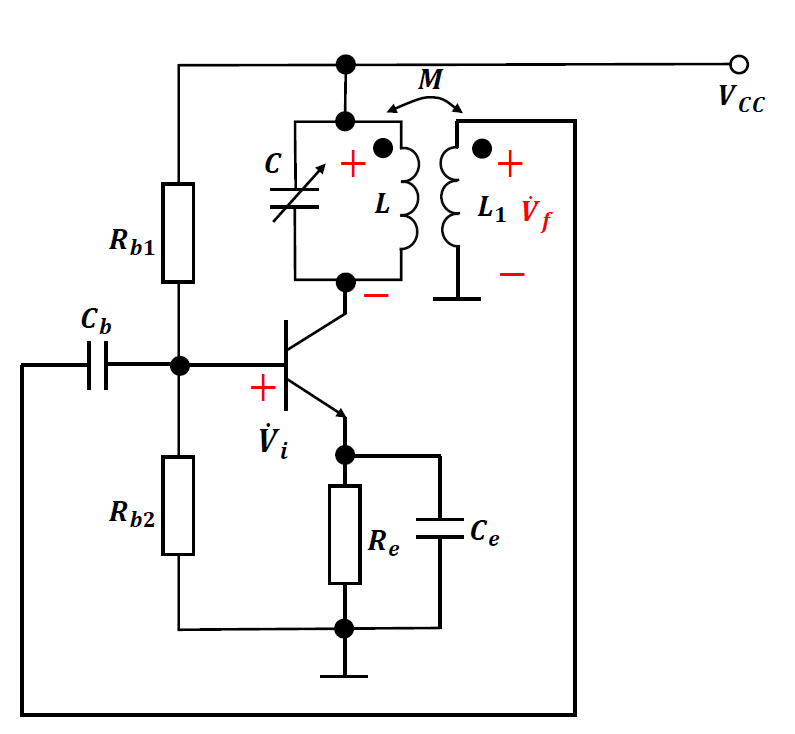
\includegraphics[width=0.33\textwidth]{osc_lc_collector.png}
  \caption{调集电路}
  \end{figure}

\section{三端振荡器}
\textbf{有源器件} (BJT)三个电极分别于\textbf{振荡回路}的三个端点\textbf{交流}相连. \\
\textbf{如何画交流等效电路}
\begin{itemize}
  \item 直流电阻开路
  \item 电感开路 (高频扼流圈开路)
  \item 电容短路
  \begin{itemize}
    \item 旁路电容短路
    \item 耦合电容短路
    \item 电源滤波电容短路
  \end{itemize}
\end{itemize}
\subsection{三端式振荡器的组成法则}
用于判断相位平衡条件. 
\begin{figure}[H]
  \centering
  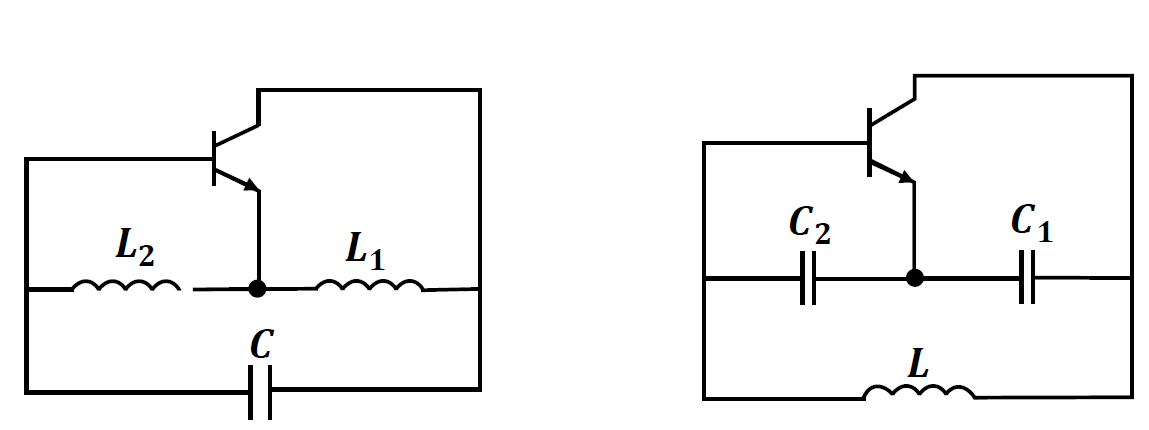
\includegraphics[width=1\textwidth]{osc_X_rule_2.png}
  \caption{例子}
  \end{figure}
\begin{quotation}
  be, ce同抗件, cb反抗件
\end{quotation}
\begin{itemize}
  \item 晶体管ce之间和be之间的回路元件电抗性质相同
  \item 它们与bc回路元件的电抗性质相反
\end{itemize}
\begin{figure}[H]
\centering
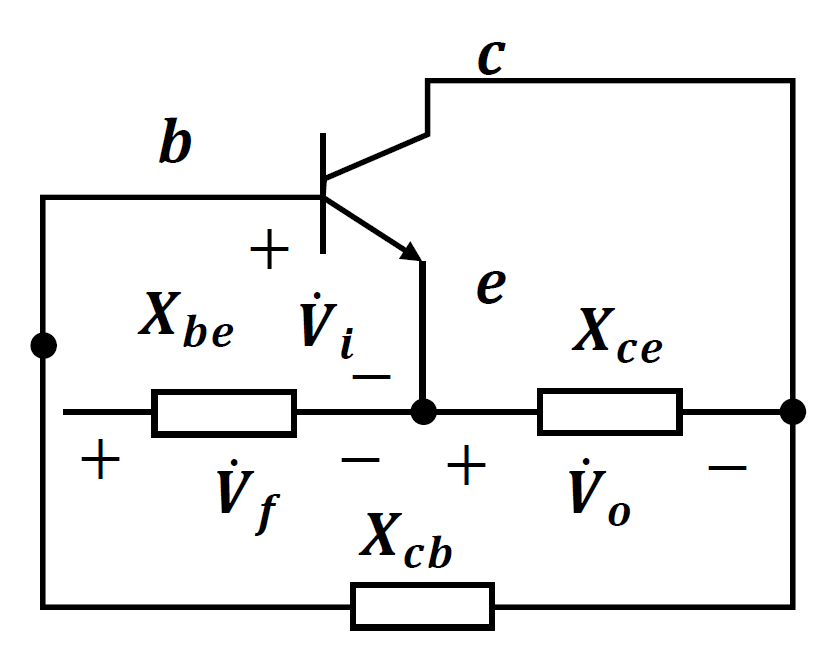
\includegraphics[width=0.5\textwidth]{osc_X_rule_1.png}
\caption{be, ce同抗, cb反抗}
\end{figure}
\subsection{Hartley Oscillator}
电感三端振荡器
\begin{figure}[H]
\centering
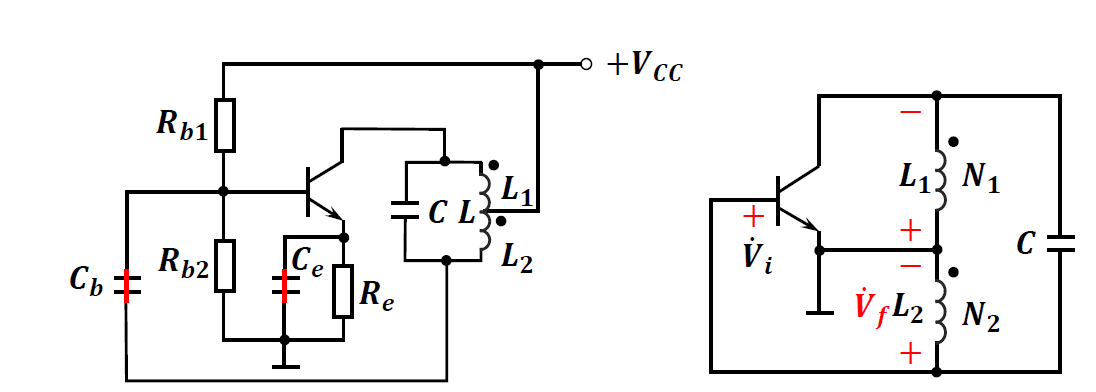
\includegraphics[width=1\textwidth]{osc_hartley.png}
\caption{哈特莱电路(左图)及其高频等效电路(右图)}
\end{figure}
\begin{align*}
  f_0&\approx \frac{1}{2\pi\sqrt{LC}}\\
  L&=L_1+L_2+2M\\
  F&=\frac{L_2+M}{L_1+M}
\end{align*}
$F$为反馈系数. \\
\textbf{优点}
\begin{itemize}
  \item 反馈较强, 容易起振
  \item 振荡频率调节方便
  \item 电容改变基本不影响电路的反馈系数
\end{itemize}
\textbf{缺点}
\begin{itemize}
  \item 振荡波形不好
  \item 振荡频率不能做得太高 
\end{itemize}
\subsection{Colpitts Oscillator}
电容三端振荡器
\begin{figure}[H]
\centering
\includegraphics[width=1\textwidth]{osc_coplitts.png}
\caption{考毕兹电路及其高频等效电路}
\end{figure}
\begin{align*}
  f_0&\approx\frac{1}{2\pi\sqrt{LC}}\\
  C&=\frac{C_1 C_2}{C_1+C_2}&&\text{就是俩电容串联}\\
  F&=\frac{C_1}{C_2}
\end{align*}
\textbf{优点}
\begin{itemize}
  \item 振荡波形好
  \item 稳定度较高
  \item 工作频率较高
\end{itemize}
\textbf{缺点}
\begin{itemize}
  \item 调电容会改变振荡频率时会改变反馈系数 (可以在L两端并联一个可变电容)
  \item 调整反馈系数时会改变振荡频率
\end{itemize}

\subsection{Clapp Oscillator}
串联型改进电容三端式振荡器\\
$C_3$一定远小于$C_1,C_2$
\begin{figure}[H]
\centering
\includegraphics[width=1\textwidth]{osc_clapp.png}
\caption{克拉泼电路及其高频等效电路}
\end{figure}
\begin{align*}
  f_0&\approx\frac{1}{2\pi\sqrt{LC_3}}\\
  C&=C_1\;\text{series}\;C_2\;\text{series}\;C_3\\
  &=\frac{C_3}{1+\frac{C_3}{C_1}+\frac{C_3}{C_2}}\approx C_3\\
  F&=\frac{C_1}{C_2}
\end{align*}
使得\textbf{振荡频率}与\textbf{反馈系数}无关. \\
\textbf{优点}
\begin{itemize}
  \item 晶体管与谐振回路是松耦合
  \item 调整$C_1,C_2$改变反馈系数, 对振荡频率影响很小
  \item 调整$C_3$改变振荡频率, 对反馈系数无影响
\end{itemize}
\textbf{缺点}
\begin{itemize}
  \item 波段覆盖范围窄
  \item 工作波段内, 输出波形随着频率变化大
\end{itemize}
\subsection{Seiler Oscillator}
并联型改进电容三端式振荡器
\begin{figure}[H]
\centering
\includegraphics[width=1\textwidth]{osc_seiler.png}
\caption{西勒电路及其高频等效电路}
\end{figure}
\begin{align*}
  f_0&\approx\frac{1}{2\pi\sqrt{L\cdot(C_3+C_4)}}&&\text{$C_3$与$C_4$并联}\\
  F&=\frac{C_1}{C_2}
\end{align*}
在满足起振条件的前提下, 尽量减小$C_3$

\section{石英晶体振荡器}
并联谐振型晶体振荡器和串联谐振型晶体振荡器
\subsection{并联石英晶体振荡器}
\subsubsection{Pierce}
并联型三端式电容 (c-b型电路\footnote{因石英晶体在BJT的cb之间得名})
\subsubsection{Miller}
并联型三端式电感 (b-e型电路\footnote{因石英晶体在BJT的be之间得名})
\subsection{串联石英晶体振荡器}
\section{寄生振荡}
\paragraph{危害}不稳定和寄生振荡使放大器产生寄生辐射,减小有用的信号功率输出,使被传输的信号产生失真。
\begin{itemize}
  \item 反馈型寄生振荡
  \begin{itemize}
    \item 内部反馈
    \item 外部反馈
  \end{itemize}
  \item 负阻型寄生振荡
  \begin{itemize}
    \item 雪崩负阻振荡: BJT工作于雪崩击穿区
    \item 过压负阻振荡: BJT工作于过压状态
  \end{itemize}
\end{itemize}
\section{小结}
\begin{figure}
\centering
\includegraphics[width=1\textwidth]{osc_map.jpg}
\caption{振荡器知识地图}
\end{figure}

\chapter{AM}
切实可行的天线尺寸
$$\text{天线几何尺寸}\geq \frac{1}{4}\times \text{信号波长}$$
高频窄带
\begin{figure}[h]
  \centering
  \begin{tikzpicture}
    \tikzset{
      box/.style={draw, rectangle, fill=blue!20, rounded corners, minimum height=3em, node distance=3cm},
      osc/.style={draw, circle, fill=green!20, minimum height=3em, node distance=3cm},
      amp/.style={draw, rectangle, fill=red!20, node distance=4cm},
      line/.style={draw, -latex'}
    }
    \node [box] (mod) {Modulation};
    \node [amp, left of = mod] (mings){Modulating Signal};
    \node [osc, below of = mod] (carrier){Carrier};
    \node [amp, right of = mod] (ms){Modulated Signal};
    
    \path [line] (mings)--(mod);
    \path [line] (carrier)--(mod);
    \path [line] (mod)--(ms);
    \end{tikzpicture}
  \caption{信号的调制}
  \end{figure}
  \begin{figure}[H]
  \centering
  \resizebox*{\textwidth}{!}{
    \begin{tikzpicture}
      \tikzset{
        box/.style={draw, rectangle, fill=blue!20, rounded corners, minimum height=3em, node distance=3cm},
        osc/.style={draw, circle, fill=green!20, minimum height=3em, node distance=3cm},
        amp/.style={draw, rectangle, fill=red!20, node distance=4cm},
        mix/.style={draw, rectangle,fill=yellow!20, node distance=4cm},
        detector/.style={draw, rectangle,fill=orange!20, node distance=4cm},
        line/.style={draw, -latex'},
      }
      \node [box] (mod) {AM};
      \node [osc, below of =mod] (osc1) {OSC};
      \node [amp, right of = mod] (amp1) {Hi-freq Power AMP};
      \node [amp, right of = amp1, node distance=5cm] (amp2) {Hi-freq Small AMP};
      \node [mix, right of = amp2, node distance = 4cm] (demod) {Mixer}; 
    
      \node [amp,right of =demod] (amp3){Intermediate freq AMP};
       %\node [mix,right of =amp2] (mixer){Mixer};
      \node [osc, below of = demod] (osc2) {OSC};
      \node [detector, right of = amp3](dec){Dector};
       \node [osc, below of =dec] (osc3) {OSC};
      
      
      \path [line] (osc1)--(mod);
      \path [line] (mod)--(amp1);
      \path [line,dashed] (amp1)--node[above]{EM Wave} (amp2);
      %yshift
      \path [line] (amp2)--(demod);
      \path [line] (osc2)--(demod);
      \path [line] (demod)--(amp3);
       \path [line] (amp3)--(dec);
        \path [line] (osc3)--(dec);
      \end{tikzpicture}

  }
  \caption{调幅过程}
  \end{figure}


\section{理论过程}
调幅为线性调制
\begin{itemize}
  \item 非线性元件+滤波器
  \item 频域: 线性频谱搬移
  \item 时域: 乘上$\cos(2\pi f_0 t)$
\end{itemize}
\begin{align*}
  v_{\Omega}(t)&=V_\Omega\cdot \cos(\Omega t)&&\text{待调制信号 (假设为单频调制)}\\
  v_0(t)&=V_0\cdot\cos(\omega_0 t) &&\text{载波}\\
  v_{AM}(t)&=V_0\cdot [1+m_a\cdot \cos(\Omega t)]\cdot \cos(\omega_0 t)\\
  m_a&=\frac{k_a\cdot V_\Omega}{V_0}&&\text{调制指数}
\end{align*}
\subsection{调制指数$m_a$}
调幅系数载物理意义上为载波电压振幅的最大变化和载波电压之比. \\
一般来说$0<m_a<1$, $m_a>1$会出现相位翻转\footnote{所谓过调制}(Phase Reversal), 不可以使用包络检波. 

调幅系数如果大于1 ,调幅波的有一段时间振幅为零,这时已调波的包络产生了严重失真,出现了过量调幅
\subsection{频谱搬移}
See Section~\ref{sec:mixing}. 
\begin{figure}[H]
\centering
\begin{tikzpicture}
\coordinate (f_s) at (0,0);
\coordinate(f_p) at ($(f_s)+(1,0)$);
\coordinate(f_m) at ($(f_s)+(-1,0)$);
\coordinate (f_0) at (5,0);

\coordinate (f_i) at (4,0);
\coordinate(f_ip) at ($(f_i)+(1,0)$);
\coordinate(f_im) at ($(f_i)+(-1,0)$);

\draw [->] (0,0) node[below]{$O$}--(7,0) node[right]{$\omega$};
\draw [->] (0,0)--(0,2) node[right]{\small amplitude};
\draw [densely dashed] (0,0)--(-2,0);


%\draw [color=red] (f_s) node[below, text=black]{$f_s$}--+(0,1) node [draw=black, circle, fill=white,inner sep=1pt]{};
\draw [color=red] (f_p) node[below, text=black]{$\Omega$}--+(0,.7) node [draw=black, circle, fill=white,inner sep=0pt]{};
\draw [color=red] (f_m) node[below, text=black]{$-\Omega$}--+(0,.7) node [draw=black, circle, fill=white,inner sep=1pt]{};



\draw [color=blue] (f_i) node[below, text=black]{$\omega_0$}--+(0,1.6) node [draw=black, circle, fill=white,inner sep=1pt]{};
\draw [color=blue] (f_ip) node[below, text=black]{$\omega_0+\Omega$}--+(0,.7) node [draw=black, circle, fill=white,inner sep=1pt]{};
\draw [color=blue] (f_im) node[below, text=black]{$\omega_0-\Omega$}--+(0,.7) node [draw=black, circle, fill=white,inner sep=1pt]{};


\end{tikzpicture}
\caption{调幅的频谱搬移}
\label{fig:am_mixing}
\end{figure}

$-\Omega$在频域上没什么意义\footnote{非要说的话正的表示正方向旋转(逆时针), 负的负方向旋转}. 图~\ref{fig:am_mixing}中红色表示调制前, 蓝色表示调制后. DSB-SC就是在频域上把$\omega_0$滤掉了, SSB就只保留一条边频 (上边频或者下边频)

\subsection{功率}
\begin{align*}
  v_{AM}(t)&=V_0\cdot [1+m_a\cdot \cos(\Omega t)]\cdot \cos(\omega_0 t)\\
  &=V_0\cdot \cos(\omega_0 t)+\frac{1}{2}\cdot m_a\cdot V_0\cdot \cos(\omega_0+\Omega)+\frac{1}{2}\cdot m_a\cdot V_0\cdot \cos(\omega_0-\Omega)
\end{align*}
\begin{align*}
  P_0&=\frac{1}{2}\cdot \frac{V_0^2}{R} &&\text{载波功率}\\
  P_{\text{SSB}}&=\frac{1}{4}\cdot m_a^2\cdot P_0 &&\text{边频功率 (Single Side Band)}\\
  P_{\text{total}}&=P_\text{carrier}+2\cdot P_\text{SSB}&&\text{有两条边带}
\end{align*}
\subsection{抑制载波的双边带调幅}
Double Side Band with Suppressed Carrier (DSB-SC). \\
会出现相位反转
\subsection{单边带调幅}
Single Side Band (SSB)\\
单边带调幅信号的方法主要有滤波器法, 相移法以及修正的移相滤波法. 
\subsection{残留边带调幅}
Vestigial Sideband (VSB)

\section{高电平调幅电路}
\subsection{集电极调幅}
利用高频功率放大器的集电极调制特性完成功放和振幅调制,功率放大器的工作状态应选\textbf{过压}状态
\subsection{基级调幅}
利用高频功率放大器的基级调制特性完成功放和振幅调制,功率放大器的工作状态应选\textbf{欠压}状态
\section{检波}
\subsection{技术指标}
主要技术指标有
\begin{itemize}
  \item 等效输入阻抗
  \item 电压传输系数
  \item 失真
\end{itemize}
\subsection{包络检波}
峰值包络检波
\begin{figure}[H]
\centering
\includegraphics[width=0.4\textwidth]{am_detector_1.png}
\caption{串联型二极管峰值包络检波}
\end{figure}


\subsection{包络检波失真}
\subsubsection{对角线切割失真 (惰性失真)}
inertia distortion;\\
滤波电容放电过慢, 使得二极管不能及时导通.
工程上
$$\Omega_\text{max}\cdot RC\geq 1.5$$ 
\subsubsection{底部切割失真 (负峰切割失真)}
negative peak clipping distortion;
\begin{figure}[H]
\centering
\includegraphics[width=0.5\textwidth]{am_distortion_peak.png}
\caption{带隔直电阻$C_c$和下级输入电阻$R_g$ (下称作$R_{i2}$)的检波电路}
\end{figure}
不产生负峰切割失真的条件
$$m_a<\frac{R_{i2}}{R+R_{i2}}$$
\subsubsection{非线性失真}
负载电阻$R$选得足够大, 则检波管的非线性特性的影响越小, 非线性失真可以被忽略. 
\subsubsection{频率失真}
\begin{align*}
  \frac{1}{\Omega_\text{min}\cdot C}&\ll R_{i2} && \text{表示\textbf{下限频率}对电容的容抗要远小于下级输入电阻$R_{i2}$}\\
  \frac{1}{\Omega_\text{max}\cdot C}&\gg R && \text{表示\textbf{上限频率}对电容的容抗要远大于R}
\end{align*}\footnote{LHS其实就是容抗$X_C$}
使得充电时间常数小, 放电时间常数大
\subsection{同步检波}
\begin{figure}[H]
\centering
\resizebox{\textwidth}{!}{

  \begin{tikzpicture}
    \tikzset{
      box/.style={draw, rectangle, fill=blue!20, rounded corners, minimum height=3em, node distance=3cm},
      osc/.style={draw, circle, fill=green!20, minimum height=3em, node distance=3cm},
      amp/.style={draw, rectangle, fill=red!20, node distance=4cm},
      line/.style={draw, -latex'}
    }
    \node [] (mod) {\Huge$\otimes$};
    \node [amp, left of = mod] (mings){Modulated Signal $v_s$};
    \node [osc, below of = mod, align=center] (carrier){Local \\Carrier\\$v_0$};
    \node [box, right of = mod] (ms){LP Filter};
    \node [amp, right of=ms](meds){Modulating Signal $v_\Omega$};
    
    \path [line] (mings)--(mod);
    \path [line] (carrier)--(mod);
    \path [line] (mod)--(ms);
    \path [line] (ms)--(meds);
    \end{tikzpicture}
}
\caption{同步检波流程}
\label{fig:sync_demod}
\end{figure}
图~\ref{fig:sync_demod}为接收端的同步检波框图. 已调制信号以DSB-SC调制, 故解调时需要加上载波; 本地载波 (Local Carrier)必须要与发送端的载波信号\textbf{同频同相}, 才有可能完全恢复原调制信号. 

\chapter{PM \& FM}
调角为非线性调制
  \begin{figure}[H]
  \centering
  \resizebox*{\textwidth}{!}{
    \begin{tikzpicture}
      \tikzset{
        box/.style={draw, rectangle, fill=blue!20, rounded corners, minimum height=3em, node distance=3cm},
        osc/.style={draw, circle, fill=green!20, minimum height=3em, node distance=3cm},
        amp/.style={draw, rectangle, fill=red!20, node distance=4cm},
        mix/.style={draw, rectangle,fill=yellow!20, node distance=4cm},
        detector/.style={draw, rectangle,fill=orange!20, node distance=4cm},
        line/.style={draw, -latex'},
      }
      \node [box] (mod) {FM};
      \node [osc, below of =mod] (osc1) {OSC};
      \node [amp, right of = mod] (amp1) {Hi-freq Power AMP};
      \node [amp, right of = amp1, node distance=5cm] (amp2) {Hi-freq Small AMP};
      \node [mix, right of = amp2, node distance = 4cm] (demod) {Mixer}; 
    
      \node [amp,right of =demod] (amp3){Intermediate freq AMP};
       %\node [mix,right of =amp2] (mixer){Mixer};
      \node [osc, below of = demod] (osc2) {OSC};
      \node [detector, right of = amp3](dec){Freq-Discrimination};
       \node [osc, below of =dec] (osc3) {OSC};
      
      
      \path [line] (osc1)--(mod);
      \path [line] (mod)--(amp1);
      \path [line,dashed] (amp1)--node[above]{EM Wave} (amp2);
      %yshift
      \path [line] (amp2)--(demod);
      \path [line] (osc2)--(demod);
      \path [line] (demod)--(amp3);
       \path [line] (amp3)--(dec);
        \path [line] (osc3)--(dec);
      \end{tikzpicture}

  }
  \caption{调频过程}
  \end{figure}
\section{调相}
\begin{align*}
  v_{\Omega}(t)&=V_\Omega\cdot \cos(\Omega t)&&\text{待调制信号 (假设为单频调制)}\\
  v_0(t)&=V_0\cdot\cos(\omega_0 t) &&\text{载波}\\
  v_{PM}(t)&=V_0\cdot \cos[\omega_0 t+k_p\cdot V_\Omega\cdot \cos(\Omega t)]\\
  &=V_0\cdot \cos[\omega_0 t+m_p\cdot \cos(\Omega t)]\\
  m_p&=k_p\cdot |v_\Omega(t)|_{\text{max}}&&\text{调相指数 (最大相位偏移)}\\
  \Delta \omega_{\text{max}}&=k_p\cdot |\frac{d v_\Omega (t) }{d t}|_{\text{max}} &&\text{最大频率偏移}\\
  \Delta \theta(t)&=k_p\cdot v_\Omega (t) &&\text{相位偏移}
\end{align*}
$k_p$为比例常数, 单位为$rad/V$, PM是以相位为参数. 
\section{调频}
\begin{align*}
  v_{\Omega}(t)&=V_\Omega\cdot \cos(\Omega t)&&\text{待调制信号 (假设为单频调制)}\\
  v_0(t)&=V_0\cdot\cos(\omega_0 t) &&\text{载波}\\
  v_{FM}(t)&=V_0\cdot \cos[\omega_0 t+k_f\cdot \int_0^t v_\Omega (t) \; dt]  &&\text{频率需要积分变为相位}\\ 
  &=V_0\cdot \cos[\omega_0 t+\frac{k_f V_\Omega}{\Omega}\cdot \sin(\Omega t)]\\
  &=V_0\cdot\cos[\omega_0 t+m_f\cdot sin(\Omega t)]\\
  m_f&=k_f\cdot |\int_0^t v_\Omega (t) \; dt|_{\text{max}}&&\text{调频指数 (最大相位偏移)}\\
  \Delta \omega_m&=k_f\cdot |v_\Omega(t)|_{\text{max}} &&\text{最大频率偏移}\\
  \Delta \theta(t)&=k_f\cdot \int_0^t v_\Omega (t) \; dt &&\text{相位偏移}
\end{align*}
不管是FM还是PM, 其调频/相指数均为最大相位偏移. 
\section{调频与调相之间的关系}
% Table generated by Excel2LaTeX from sheet 'Sheet1'
% Table generated by Excel2LaTeX from sheet 'Sheet1'
\begin{table}[htbp]
  \centering
  \resizebox{\textwidth}{!}{

    \begin{tabular}{c|c|c}
          & PM    & FM \\
          \hline
    角频率偏移  &   $\Delta\omega(t)=k_p\cdot \frac{d \,v_\Omega(t) }{d t}$   & $\Delta\omega(t)=k_f\cdot v_\Omega(t)$ \\
    相位偏移\footnotemark   &  $\Delta \theta(t)=k_p\cdot v_\Omega(t)$     & $\Delta \theta(t)=k_f\int_0^t v_\Omega(t)\;dt$ \\
    最大相位偏移 &   $\Delta\theta_\text{max}=k_p\cdot |v_\Omega(t)|_\text{max}$    & $\Delta\theta_\text{max}=k_f |\int_0^t v_\Omega(t)\;dt|_\text{max}$ \\
    最大角频率偏移 &   $\Delta\omega_\text{max}=k_p |\frac{d\, v_\Omega(t) }{d t}|_\text{max}$    &  $\Delta\omega_\text{max}=k_f\cdot |v_\Omega(t)|_\text{max}$\\
    调制指数 \footnotemark &   $m_p=k_p\cdot V_\Omega$    & $m_f=\frac{k_f V_\Omega}{\Omega}$ \\
    \hline
    被调波   & \multicolumn{2}{c}{$v_\Omega(t)=V_\Omega\cos(\Omega t)$} \\
    载波    & \multicolumn{2}{c}{$v_\text{carrier}(t)=V_0\cos(\omega_0 t)$} \\
    \hline
    已调波   & $v_\text{PM}=V_0\cdot \cos(\omega_0t+m_p\cdot\cos\,\Omega t)$ & $v_\text{FM}=V_0\cdot \cos(\omega_0 t+m_f\cdot \sin\,\Omega t)$\\
    \hline
    最大频率偏移\footnotemark  & \multicolumn{2}{c}{$\Delta f_m=m\cdot F$} \\
    \end{tabular}%
  }
    \caption{PM与FM关系表}
    
\end{table}%
\footnotetext[1]{相位偏移就是丢到已调波表达式的$\cos$里边的玩意. }
\footnotetext[2]{说白了就是最大相位偏移. 这里为了方便起见使用了单频率调制的情况, 即被调制波为$v_\Omega(t)=V_\Omega\cdot\cos(\Omega t)$}
\footnotetext[3]{$F=\frac{\Omega}{2\pi}$为载波的频率, $m$为调制指数 (FM或者PM均可)}



\begin{figure}[H]
\centering

\begin{tikzpicture}
  \tikzset{
    box/.style={draw, rectangle, fill=blue!20, rounded corners, minimum height=3em, node distance=3cm},
    osc/.style={draw, circle, fill=green!20, minimum height=3em, node distance=3cm},
    amp/.style={draw, rectangle, fill=red!20, node distance=2cm},
    mix/.style={draw, rectangle,fill=yellow!20, node distance=4cm},
    detector/.style={draw, rectangle,fill=orange!20, node distance=4cm},
    line/.style={draw, -latex'},
  }
  \node [box] (fm) {PM};
    \node [amp, left of = fm, align=center] (int){int \\ $\int\cdot\; dt$};
  \node [left of =int, node distance=2cm](vw){$v_\Omega(t)$};
\node [right of = fm, node distance=2cm](vfm){$v_{\text{FM}}(t)$};
  
  \path [line] (vw)--(int);
  \path [line] (int)--(fm);
    \path [line] (fm)--(vfm);
  
  \end{tikzpicture}

\caption{调相变调频}
\end{figure}

\begin{figure}[H]
  \centering
\begin{tikzpicture}
  \tikzset{
    box/.style={draw, rectangle, fill=blue!20, rounded corners, minimum height=3em, node distance=3cm},
    osc/.style={draw, circle, fill=green!20, minimum height=3em, node distance=3cm},
    amp/.style={draw, rectangle, fill=red!20, node distance=2cm},
    mix/.style={draw, rectangle,fill=yellow!20, node distance=4cm},
    detector/.style={draw, rectangle,fill=orange!20, node distance=4cm},
    line/.style={draw, -latex'},
  }
  \node [box] (fm) {FM};
    \node [amp, left of = fm, align=center] (int){diff \\ $\frac{d \cdot }{d t}$};
  \node [left of =int, node distance=2cm](vw){$v_\Omega(t)$};
\node [right of = fm, node distance=2cm](vfm){$v_{\text{PM}}(t)$};
  
  \path [line] (vw)--(int);
  \path [line] (int)--(fm);
    \path [line] (fm)--(vfm);
  
  \end{tikzpicture}

\caption{调频变调相}
\end{figure}
\begin{itemize}
  \item 调频波可以看作是调制信号$v_\Omega$经过积分之后的调相波
  \item 调相波可以看作是调制信号$v_\Omega$经过微分之后的调频波
\end{itemize}
\subsection{频率}
$m_f$越大, 具有较大振幅的边频率就越多. \\
$\Delta f_{\text{max}}=m\cdot F$最大频率偏移, 又被称作偏频. 
\paragraph{有效频带宽度} 单频调制时 $v_\Omega(t)=V_\Omega\cos(\Omega t)$
\begin{align*}
  \text{Bandwidth}_\text{调角}&=2\cdot (\Delta f_{\text{max}}+F)\\
  \Delta f_{\text{max}}&= m_f\cdot F\\
  &=m_p\cdot F\\
  F&=\frac{\Omega}{2\pi}\\
  m_f&=\frac{k_f\cdot V_\Omega}{\Omega}\\
  m_p&=k_p\cdot V_\Omega
\end{align*}
对于FM, 当调制信号频率F变化时, 调频指数$m_f$与F成反比, 最大频偏不变, 带宽基本不变. (恒带调制)
\subsection{功率}
\begin{align*}
  P_\text{调角}=\frac{1}{2}\cdot\frac{V_0^2}{R_L}
\end{align*}
将原来载波功率重新分配到各个边频上, 总功率不变. 
\subsection{输入为正弦}
假设被调信号为$v_\Omega=V_\Omega\cdot \sin(\Omega t)$则FM波为
$$v_\text{FM}=V_0\cdot \cos[\omega_0 t- m_f\cdot\cos(\Omega t)]$$
其实就是把$\sin(\Omega t)$积分变成$-\cos(\Omega t)$, 记得乘上调制系数. \\
PM波就直接乘上调制系数不用积分了. 
\section{调角理论小结}
\begin{figure}[H]
\centering
\includegraphics[width=\textwidth]{fm_map.jpg}
\caption{知识地图}
\end{figure}

\section{调频电路}
\subsection{直接调频}
直接调频的优点是频偏大
\subsubsection{变容二极管}
\subsubsection{晶体振荡器 (Pierece)}
\subsection{间接调频}
间接调频的优点是中心频率稳定度高
\section{鉴频}
\subsection{鉴频技术指标}
\subsubsection{鉴频跨导}
\begin{figure}[H]
\centering
\includegraphics[width=0.4\textwidth]{fm_dis_trans_con.png}
\caption{鉴频特性曲线}
\end{figure}
$$S=\frac{\Delta v_0}{\Delta f}|_{f=f_0}$$
中心频率附近, 单位频率偏移引起的输出电压的变化量. \\
S越大, 曲线斜率越大, 单位解调能力就越强
\subsubsection{鉴频带宽}
$2\Delta f_{max}$又被称作线性范围, 鉴频特性曲线中接近直线段的变化频率范围. \\
不失真时解调的所允许的频率变化范围. 
\subsubsection{鉴频输入灵敏度}
值越小灵敏度越高
\subsection{波形变换鉴频}
\begin{figure}[H]
\centering
\includegraphics[width=0.6\textwidth]{fm_fm_am.png}
\caption{FM$\rightarrow$FM-AM}
\end{figure}
\subsubsection{相位鉴频器}
phase discriminator
\begin{figure}[H]
\centering
\includegraphics[width=1\textwidth]{fm_phase_discr.png}
\caption{相位鉴频器电路}
\end{figure}
\textbf{缺陷} 有寄生调幅, 需要增加限幅器. 
\subsubsection{比例鉴频器}
ratio detector
\begin{figure}[H]
\centering
\includegraphics[width=1\textwidth]{fm_ratio_dector.png}
\caption{比例鉴频器电路}
\end{figure}
自带限幅器
\subsection{相移乘法鉴频}
FM$\rightarrow$FM-PM
\end{document}